\chapter{Software Quality}

\section{Define aspects of software defects and defect management alternatives}

\textblue{Defect} = some problem with the software
\begin{itemize}
    \item[$\hookrightarrow$] (Human) Error : a mistake in performing some software activities
    \item[$\hookrightarrow$] Fault : a defect in the product
    \item[$\hookrightarrow$] Failure : a departure from the system's required behaviour
    \item[] \textblue{High quality} $\approx$ low defect
    \item[] \textblue{Quality problem} $\approx$ defect impact
\end{itemize}

\textblue{Dealing with defects :}

\begin{minipage}{0.48\textwidth}
\begin{enumerate}
        \item \textblue{Defect prevention} :
        \begin{itemize}
            \item  Prevent faults from being injected
            \item  Error blocking, error source removal
        \end{itemize}
        \item \textblue{Defect removal} :
        \begin{itemize}
            \item  Remove faults
            \item  Inspection (find faults), testing (find failures from faults
        \end{itemize}
        \item \textblue{Defect containment} :
        \begin{itemize}
            \item  Keep failures local, reduce failure impact
            \item  Fault-tolerance, failure containment
        \end{itemize}
    \end{enumerate}
\end{minipage}
\hfill
\begin{minipage}{0.48\textwidth}
    \begin{figure}[H]
        \centering
        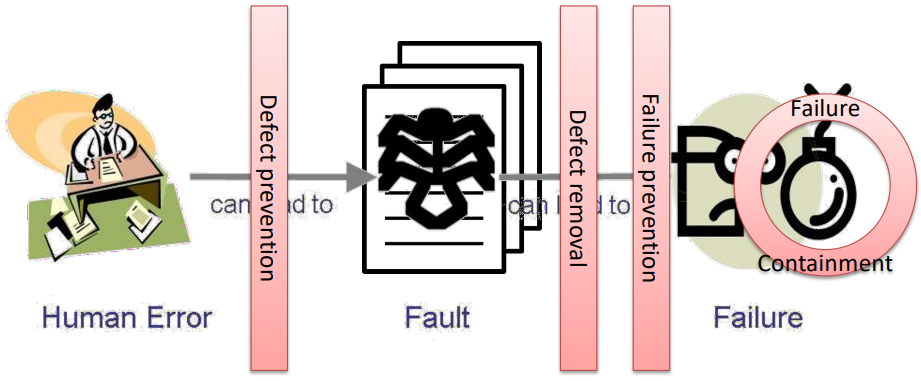
\includegraphics[width=\textwidth,keepaspectratio]{dealing_with_defects}
    \end{figure}
\end{minipage}

\section{Discuss different software quality characteristics and perspectives}

\textblue{What is good software ? What is quality ?}
\begin{itemize}
    \item \textit{Transcendental} view : an ideal that we thrive to but cannot attain
    \item \textit{User} view : fitness for purpose, reliability, absence of defects
    \item \textit{Manufacturing} view : conformance to the process
    \item \textit{Product} view : showing good inherent characteristics
    \item \textit{Value-based} view : how much the customer is willing to pay for it
\end{itemize}

Quality models relate the user's external view to the developer's internal view :

\begin{minipage}[t]{0.48\textwidth}
    \textblue{Consumers} $=$
    \begin{enumerate}
        \item \textblue{Client} : pay for the development
        \item \textblue{User} of software
        \item \textblue{Customers} : buy  after development
    \end{enumerate}
    Expect \textblue{external} qualities : 
    \begin{enumerate}
        \item good enough for the price
        \item fit‐for‐use, doing the right things
        \item conformance, doing things right
    \end{enumerate}
\end{minipage}
\hfill
\begin{minipage}[t]{0.48\textwidth}
    \textblue{Producers} $=$ Developer
    
    Expect \textblue{internal} qualities : 
    \begin{enumerate}
        \item good enough for the cost
        \item maintainable
        \item interoperable
        \item modular
    \end{enumerate}
\end{minipage}

\begin{minipage}[t]{0.48\textwidth}
    $\Rightarrow$ Judge \textblue{external} characteristics : number and type of \textblue{failures}
\end{minipage}
\hfill
\begin{minipage}[t]{0.48\textwidth}
    $\Rightarrow$ Judge \textblue{internal} characteristics : number and type of \textblue{faults}
\end{minipage}

\newpage
\section{Define correctness, reliability, safety and robustness}

These are "dependability properties" (Correctness properties are \textit{undecidable} for non-trivial programs): 
\begin{itemize}
    \item  \textblue{Correctness:} a program is correct if it is consistent with its specification (seldom practical for non-trivial systems)
    \item  \textblue{Reliability:} likelihood of correct function for some "unit" of behaviour, relative to a specification and usage profile, statistical approximation to correctness (100\% reliable = correct)
    \item  \textblue{Safety:} preventing hazards, which are system-specific undesirable behaviours
    \item  \textblue{Robustness:} acceptable (degraded) behaviour under extreme conditions
\end{itemize}

\begin{figure}[H]
    \centering
    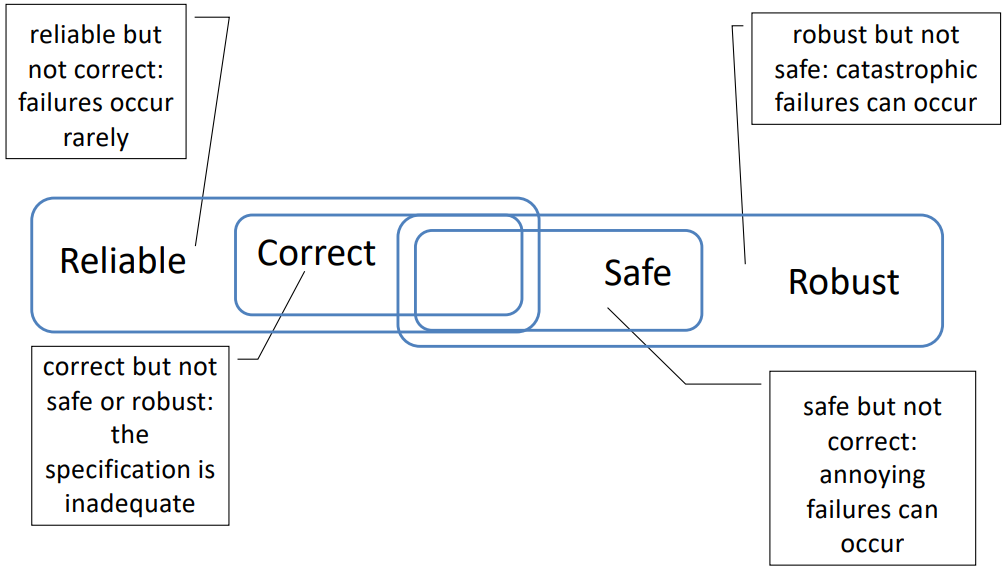
\includegraphics[width=0.7\textwidth,keepaspectratio]{realation_among_dq}
\end{figure}

\chapter{Software Development Process}

\section{Define software verification and validation}

\begin{minipage}[t]{0.48\textwidth}
    \textblue{Verification} $=$ does the software system meets the requirements specs ? Are we building the software right ?
    
    $\hookrightarrow$ Application conform to specifications
\end{minipage}
\hfill
\begin{minipage}[t]{0.48\textwidth}
    \textblue{Validation} $=$ does the software system meets the user's real need ? Are we building the right software ?
    
    $\hookrightarrow$ Specifications accurately reflects the customer's needs
\end{minipage}

\begin{minipage}[t]{0.48\textwidth}
    \textblue{Techniques} :
    \begin{enumerate}
        \item Consistency / Completeness / Reachability checks
        \item Model checking
        \item Mathematical proofs
    \end{enumerate}
\end{minipage}
\hfill
\begin{minipage}[t]{0.48\textwidth}
    \textblue{Techniques} :
    \begin{enumerate}
        \item Modelling
        \item Scenarios
        \item Prototypes
        \item Simulation
        \item[] ...
    \end{enumerate}
\end{minipage}

\section{Describe a software development process and how verification and validation activities fit into this process}

\textblue{Classic approach} : Requirement $\rightarrow$ Specifications $\rightarrow$ Design $\rightarrow$ Coding $\rightarrow$ Testing $\rightarrow$ Release

\textblue{Variation} : Waterfall, iterative, spiral, agile, ...

\begin{figure}[H]
    \centering
    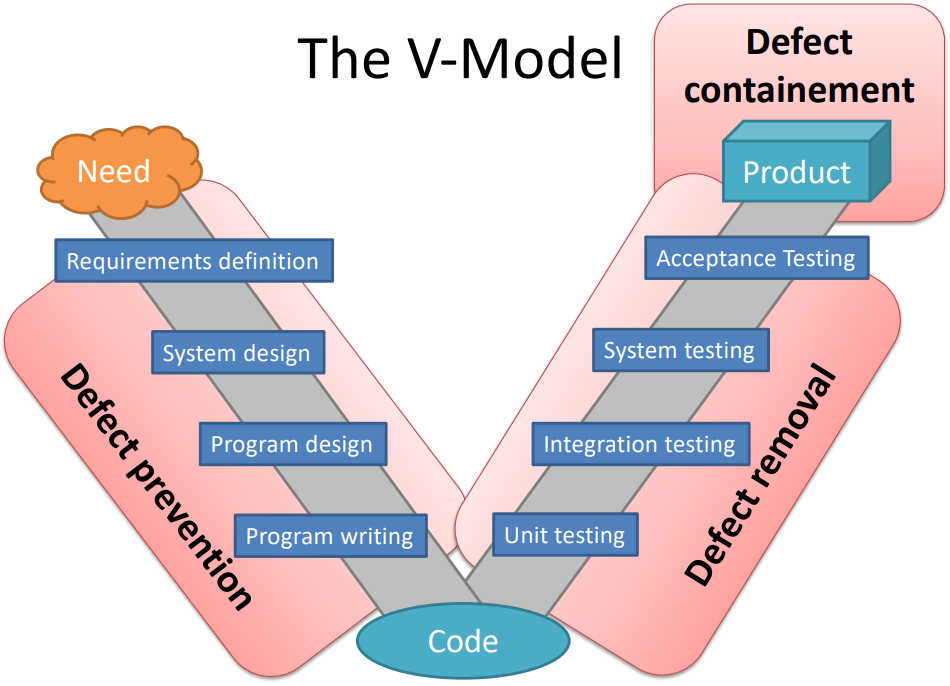
\includegraphics[width=0.48\textwidth,keepaspectratio]{v_model}\hfill
    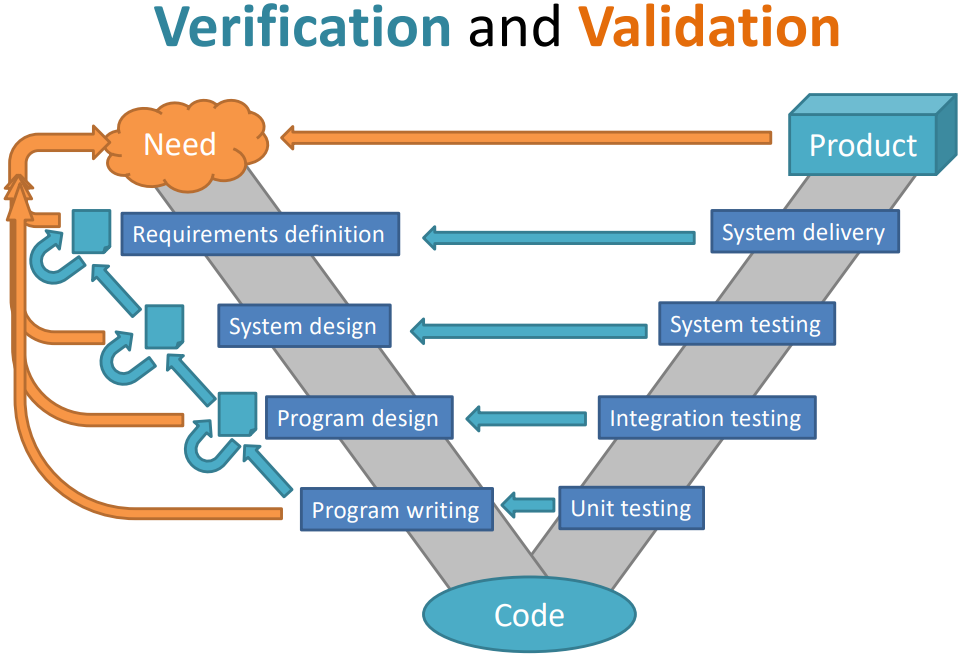
\includegraphics[width=0.48\textwidth,keepaspectratio]{v_v}
\end{figure}

\newpage
\section{Describe different types of software quality assurance activities}

\begin{enumerate}
    \item \textblue{Testing}
    \begin{itemize}
        \item Executing late in development
        \item Generate tests as early as possible
        \begin{itemize}
            \item Tests generated independently from code, when the specifications are fresh in the mind of analysts
            \item Generation of test cases may highlight inconsistencies and incompleteness of the corresponding specifications
            \item Tests may be used as compendium of the specifications by the programmers
        \end{itemize}
    \end{itemize}
    \item \textblue{Inspection}
    \begin{itemize}
        \item Can be applied to essentially any document (requirements statements, architectural and detailed design documents, test plans and test cases, program source code)
        \item May also have secondary benefits (spreading good practices, instilling shared standards of quality)
        \item Takes a considerable amount of time
        \item Re-inspecting a changed component can be expensive
        \item Used primarily where other techniques
         \begin{itemize}
            \item are inapplicable
            \item do not provide sufficient coverage
        \end{itemize}
    \end{itemize}
    \item \textblue{Automatic Static Analysis}
    \begin{itemize}
        \item More limited in applicability : can be applied to some formal representations of requirements models but not to natural language documents
        \item Are selected when available
        \begin{itemize}
            \item Substituting machine cycles for human effort makes them particularly cost-effective
        \end{itemize}
    \end{itemize}
        \item \textblue{Computer-Aided Verification}
    \begin{itemize}
        \item \textblue{Model checking} : exhaustive search of a specification's execution space
        \begin{itemize}
            \item Applicable to behaviour models (e.g. statecharts, Petri nets)
            \item Check state conditions, temporal logic, compare models
        \end{itemize}
        \item \textblue{Theorem proving} : prove Specifications AND Assumptions IMPLY Requirements
        \begin{itemize}
            \item Using built-in theories, inference rules, decision procedures
        \end{itemize}
    \end{itemize}
    \item \textblue{Improving the Process}
    \begin{itemize}
        \item Long lasting errors are common
        \item It is important to structure the process for
        \begin{itemize}
            \item the most critical persistent faults
            \item tracking them to frequent errors
            \item adjusting the development and quality processes to eliminate errors
        \end{itemize}
        \item Feedback mechanisms are the main ingredient of the quality process for identifying and removing errors
    \end{itemize}
\end{enumerate}

\chapter{Behaviour models}

\section{Define state models}

\textblue{Models} = \textit{abstraction} of the system (removes irrelevant attributes or details via an abstraction function)
\begin{itemize}
    \item Represent a system, an artefact, a design
    \item Analyse a system, an artefact, a design
    \begin{itemize}
        \item before the system is built
        \item easier to analyse/check/test than the actual system
    \end{itemize}
    \item \textblue{Properties} : Compact, Predictive, Semantically meaningful and Sufficiently general
\end{itemize}

\textblue{State models}
\begin{itemize}
    \item \textblue{Program execution} = sequence of states and transitions
    \begin{itemize}
        \item \textblue{States} : control + data (Location + variables, stack, heap)
        \item \textblue{Transitions} : actions (ops, instructions)
    \end{itemize}
    \item \textblue{State Space} :
    \begin{itemize}
        \item \textblue{Full} (all possible values)
        \item \textblue{Reachable} (from initial states)
    \end{itemize}
\end{itemize}

Essentially \textblue{infinite}\\
\textblue{Finite models} of program execution $\Rightarrow$ abstraction
\begin{enumerate}
    \item Execution is \textblue{coarsened} (fewer steps)
    \item \textblue{Nondeterminism} is introduced
\end{enumerate}

\section{Describe control flow graphs and their constituents}

\textblue{Abstraction} : set of program locations (PC) $\rightarrow$ finite number of locations

\textblue{Control Flow Graph (CFG)} :
\begin{itemize}
    \item \textblue{Nodes} = regions of source code (basics blocks)
    \begin{itemize}
        \item Basic block: maximal program region with a single entry and single exit point
        \begin{enumerate}
            \item Often several statements in one blocks
            \item Sometimes one statement in several blocks
        \end{enumerate}
    \end{itemize}
    \item \textblue{Edge} = possibility that execution proceeds from the end of one region to the beginning of another
\end{itemize}

\begin{figure}[H]
    \centering
    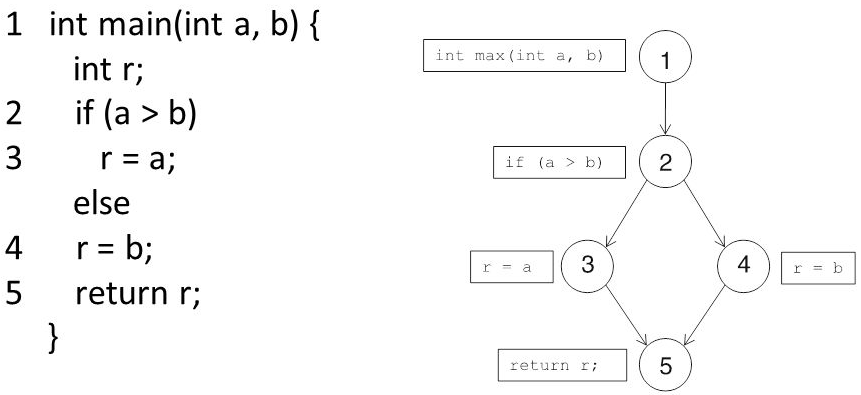
\includegraphics[width=0.6\textwidth,keepaspectratio]{cfg_example}
\end{figure}

$\Rightarrow$ \textblue{Intra-procedural} (ignore calls). May not cover some flows (e.g : exceptions are not covered)

\textblue{Linear Code Sequence and Jump (LCSJ)}: Subpaths from one branching point to another (jumps)

\section{Describe call graphs and discuss context-sensitive analysis}

\textblue{Call graphs} : 
\begin{itemize}
    \item Nodes represent procedures
    \item Edges represent calls relation
\end{itemize}

$\Rightarrow$ \textblue{Inter-procedural} 

\begin{figure}[H]
    \centering
    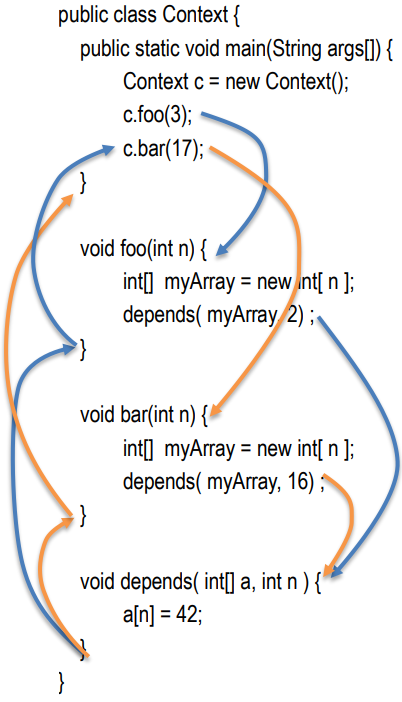
\includegraphics[width=0.23\textwidth,keepaspectratio]{call_graph_code}
\end{figure}

\begin{minipage}[t]{0.48\textwidth}
    Context-Insensitive Call Graph
    \begin{figure}[H]
        \centering
        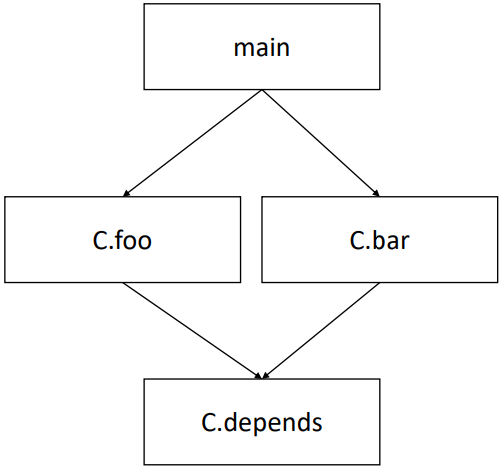
\includegraphics[width=0.6\textwidth,keepaspectratio]{call_graph_CI}
    \end{figure}
\end{minipage}
\hfill
\begin{minipage}[t]{0.48\textwidth}
    Context-Sensitive Call Graph
    \begin{figure}[H]
        \centering
        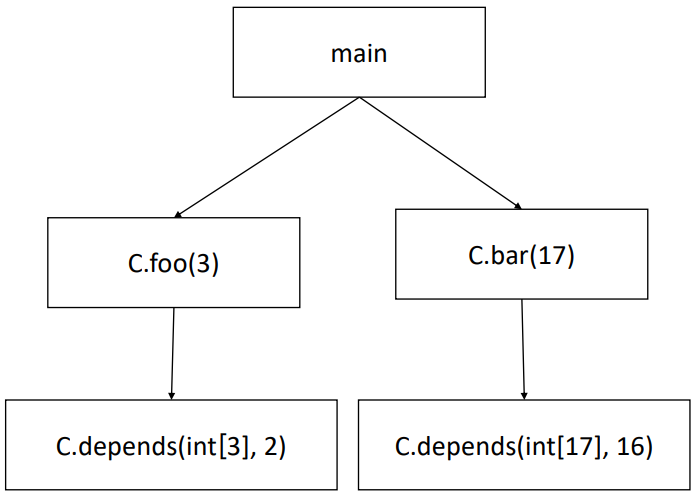
\includegraphics[width=0.8\textwidth,keepaspectratio]{call_graph_CS}
    \end{figure}
    Keep information about \textblue{calling context}, may infer that depends does not violate bounds of $a[...]$
\end{minipage}

\textblue{Context-sensitive analysis}:  the number of contexts grows exponentially with the depth of the calls :
\begin{itemize}
    \item $\#C \approx \#P^{depth}$
    \item Where $\#C$ is number of contexts and $\#P$ the number of procedures
\end{itemize}

\newpage
\section{Describe finite state machines and discuss abstraction}

\begin{itemize}
    \item  \textblue{Nodes} = states (finite number)
    \item  \textblue{Edges} = transitions
    \begin{itemize}
        \item Labelled with condition, operation, event
        \item Input/output : Mealy Machine
    \end{itemize}
    \item Used as \textblue{specifications} of allowed behaviour
\end{itemize}

For example, a transition diagram (Mealy machine) or a state-transition table.

\textblue{Abstraction function} : checking correctness with respect to the written program (Finite State Machine accurately represents program behaviour $\equiv$ program correctly implements FSM abstraction).

\textblue{Abstract} (function) : takes a program state returns a FSM state

\textblue{Example} :
\begin{figure}[H]
    \centering
    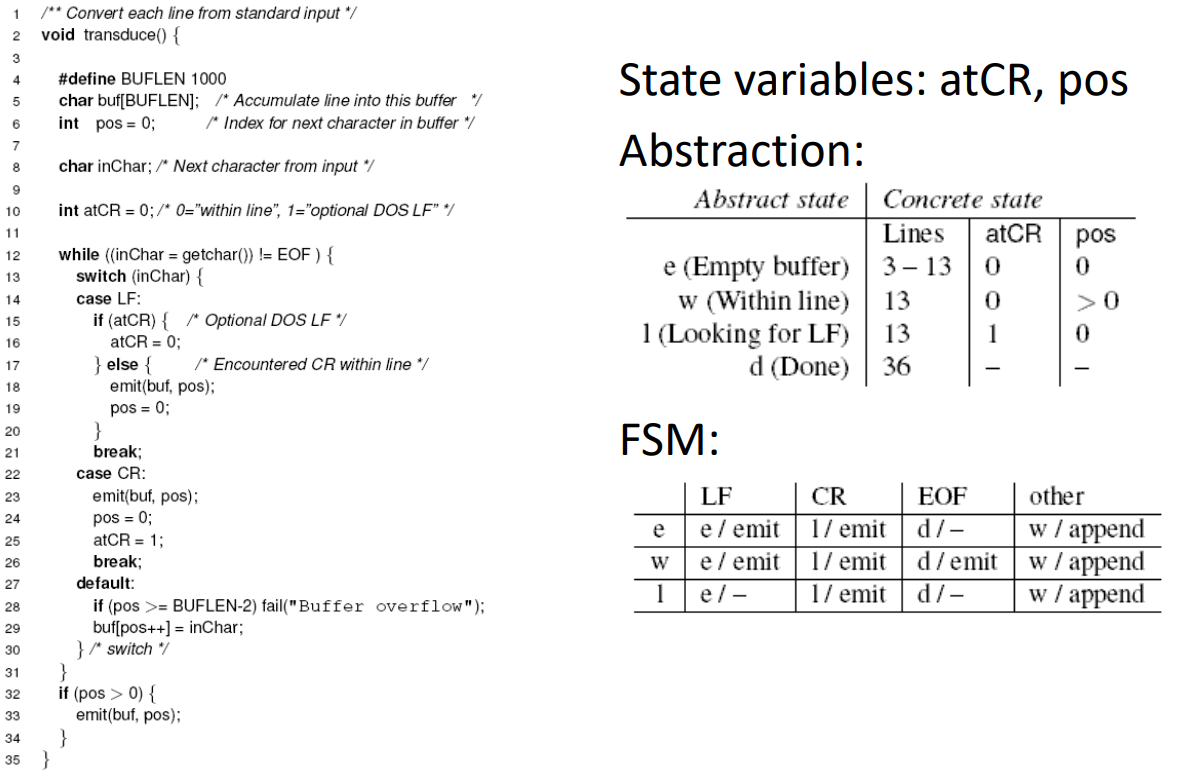
\includegraphics[width=\textwidth,keepaspectratio]{abstraction_example}
\end{figure}

\chapter{Data models}

\section{Define data dependence based on def-use pairs}

\begin{minipage}[t]{0.48\textwidth}
    \begin{enumerate}
        \item \textblue{Def} :

        Point where a variable gets a value (declaration, initialization, assignment or value received by parameter)
    \item \textblue{Use} :

    Point where a value from a variable is used (expression, conditional statement, parameter passing, returns)
    \item[$\Rightarrow$] \textblue{Def-Use pair} : Pair of points
    \begin{itemize}
        \item from where a value is produced
        \item to where that value is used
    \end{itemize}
\end{enumerate}
\end{minipage}
\hfill
\begin{minipage}[t]{0.48\textwidth}
\begin{figure}[H]
    \centering
    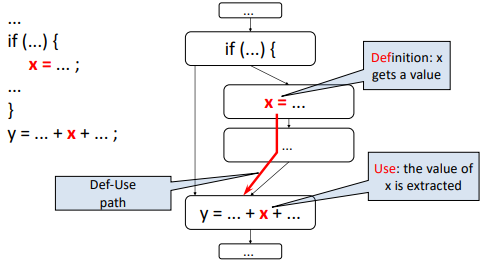
\includegraphics[width=\textwidth,keepaspectratio]{def_use}
\end{figure}
\end{minipage}

$\Rightarrow$ \textblue{Data dependence based on def-use pairs} : Where does this value of x come from? What would be affected by changing this? ...

\section{Describe data dependence and control dependence graphs}

\begin{minipage}[t]{0.48\textwidth}
    \textblue{Data dependence graph} :
    \begin{enumerate}
        \item \textblue{Nodes} :
        
        Program regions as in the control flow graph
        \item \textblue{Edges} :
        
        \textblue{Def-use pairs} labelled with the variable name
        \vspace{11pt}
        \item[$\Rightarrow$] \textblue{Data dependence} :
        
        P2 depends on P1 iff data values used in P2 can be defined in P1 (P1 is a         \textblue{definition point}, P2 is an \textblue{use point})
    \end{enumerate}
\end{minipage}
\hfill
\begin{minipage}[t]{0.48\textwidth}
    \textblue{Control dependence graph} :
    \begin{enumerate}
        \item \textblue{Nodes} :
        
        Program regions as in the control flow graph
        \item \textblue{Edges} :
        
        From \textblue{entry / branching} points to controlled blocks
        \item[$\Rightarrow$] \textblue{Control dependence} :
        
        P2 depends on P1 iff P1 controls whether P2 executes (P1 is an \textblue{entry / branching point}, P2 is \textblue{any point})
    \end{enumerate}
\end{minipage}

\begin{minipage}{0.48\textwidth}
    \begin{figure}[H]
        \centering
        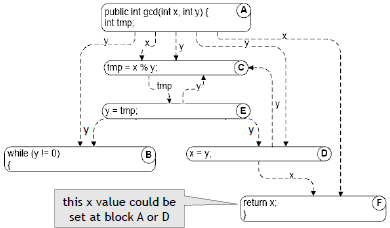
\includegraphics[width=\textwidth,keepaspectratio]{data_dep_g}
    \end{figure}
\end{minipage}
\hfill
\begin{minipage}{0.48\textwidth}
    \begin{figure}[H]
        \centering
        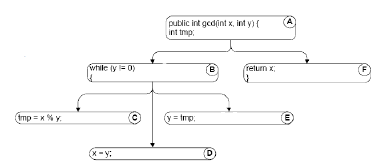
\includegraphics[width=\textwidth,keepaspectratio]{control_dep_g}
    \end{figure}
\end{minipage}

The difference with control flow is that blocks of CFG only follow other blocks but do not depends on them. Either of these blocks could be executed in either order.

\newpage
\section{Explain the general principle of dataflow analyses based on worklist algorithms, and the particular case of computing reaching definitions}

\textblue{Reaching definition}

\begin{minipage}{0.64\textwidth}
    Let :
    \begin{enumerate}
        \item $v_d, v_e$ definitions of variables $v$ at points $d,e$
        \item $u$ a point where $v$ is used
        \item[$\Rightarrow$] Definition $v_d$ \textblue{reaches} $u$ ($v_d$ is a \textblue{reaching definition} at $u$) iff 
        \begin{enumerate}
            \item There is at least one control flow path from $d$ to $u$
            \item There is no intervening definition of $v$ on the path
        \end{enumerate}
        \item[$\Rightarrow$] $v_e$ \textblue{kills} $v_d$ iff it is on a control path from $d$
        \item[$\Rightarrow$] $(d,u)$ is a \textblue{def-use pair} of $v$ iff $v_d$ \textblue{reaches} $u$
    \end{enumerate}
\end{minipage}
\hfill
\begin{minipage}{0.35\textwidth}
    \begin{figure}[H]
        \centering
        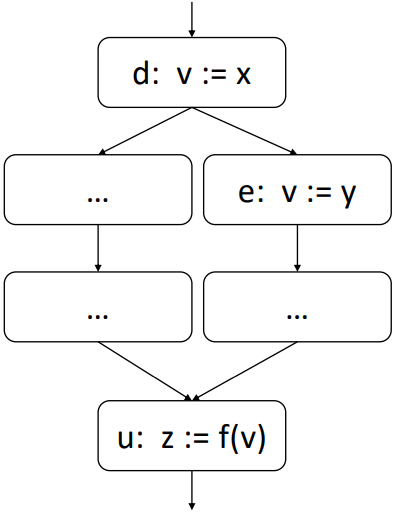
\includegraphics[width=0.5\textwidth,keepaspectratio]{reaching_def}
    \end{figure}
\end{minipage}

\textblue{Calculating Def‐Use Pairs}

Even with loop‐free paths, the number of paths in a graph can be \textblue{exponentially larger} than the number of nodes and edges. So we don’t want to search every individual path but we want to summarize the reaching definitions at a node over all the paths reaching that node.

\textblue{DF Algorithm} :

\begin{itemize}
    \item \textblue{Goal} : compute reaching definitions at node $n$
    \item Suppose that node $p$ is an immediate predecessor of node $n$
    \begin{itemize}
    \item If $p$ can assign variable $v$, then $v_p$ reaches $n$. We say the definition $v_p$ is generated at $p$
    \item If a definition $v_d$ reaches $p$, and if $v$ is not redefined at $p$, then $v_d$ reaches $n$.
    \end{itemize}
    \item $Reach(n) =$ set of definitions that reach $n$
    \item $ReachOut(n) =$ set of definitions that exit $n$
\end{itemize}
\begin{figure}[H]
    \centering
    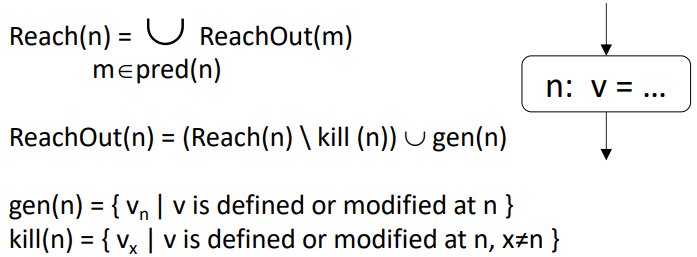
\includegraphics[width=0.5\textwidth,keepaspectratio]{reach_analysis}
\end{figure}
\begin{itemize}
    \item[$\Rightarrow$] \textblue{Recursive equations} for all nodes $n$
    \item[$\Rightarrow$] \textblue{Fixed point} computation
\end{itemize}

\textblue{Worklist Algorithm} :
\begin{minipage}{0.48\textwidth}

\end{minipage}
\begin{minted}[escapeinside=@@]{py}
foreach n @$\in$@ nodes {
    ReachOut(n) = {}
}
worklist = nodes
while worklist @$\neq$@ {} {
    n = choose (worklist)
    worklist = worklist \ {n}
    oldVal = ReachOut(n);
    Reach(n) = @$\bigcup_{m \in pred(n)}$@ ReachOut(m)
    ReachOut(n) = (Reach(n) \ kill(n)) @$\cup$@ gen(n)
    if ReachOut(n) @$\neq$@ oldVal {
        worklist = worklist @$\cup$@ succ (n)
    }
}
\end{minted}

\newpage
\textblue{Example} :
\begin{figure}[H]
    \centering
    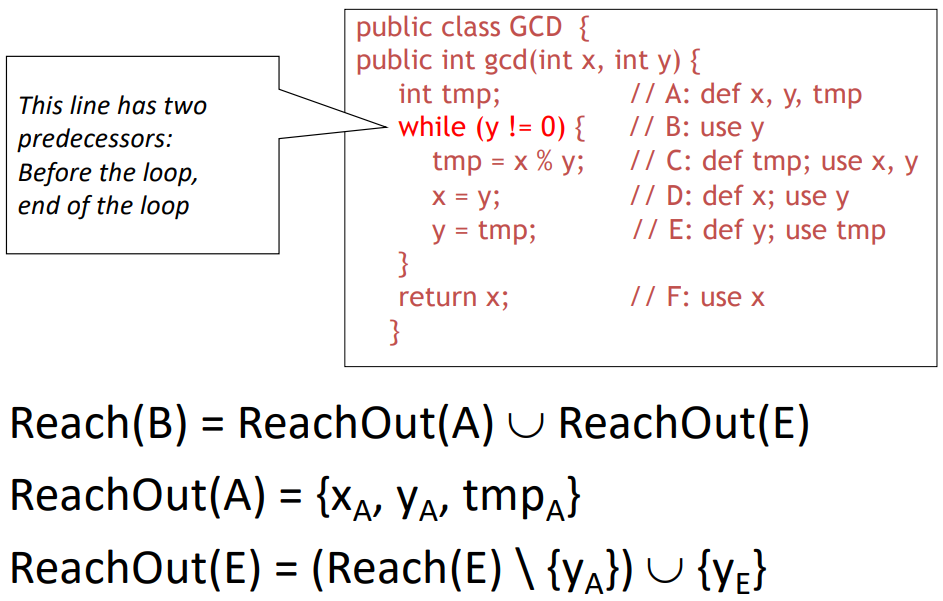
\includegraphics[width=0.6\textwidth,keepaspectratio]{worklist_ex_1}\\
    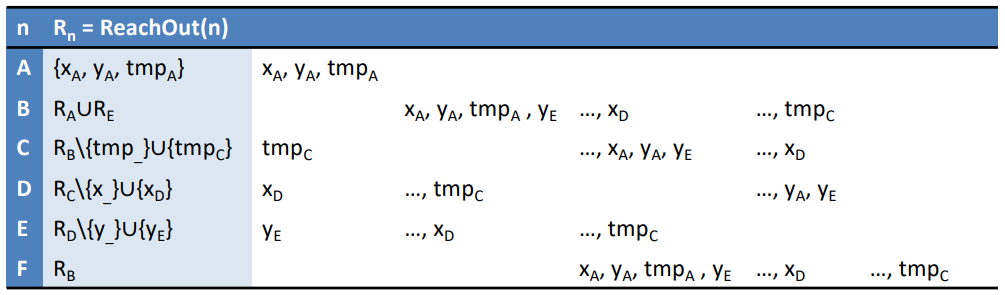
\includegraphics[width=0.7\textwidth,keepaspectratio]{worklist_ex_2}
\end{figure}

\textblue{Particular cases} :
\begin{enumerate}
    \item \textblue{Avail expressions} : expression $exp$ is \textblue{available} at node $n$ iff for all paths to $n$, $exp$ has been computed and not subsequently modified (used in compiler construction)
    \begin{figure}[H]
        \centering
        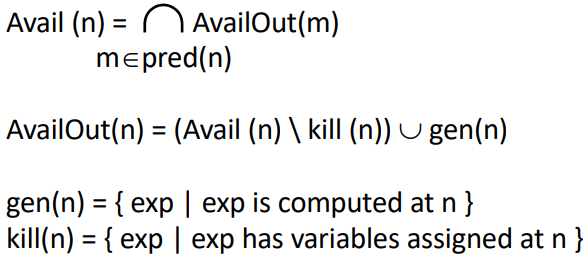
\includegraphics[width=0.4\textwidth,keepaspectratio]{avail_exp}
    \end{figure}
    \item \textblue{Live variables} : A variable $v$ is \textblue{live} at node $n$ iff on some execution path from $n$, $v$ is used before it is changed
    \begin{figure}[H]
        \centering
        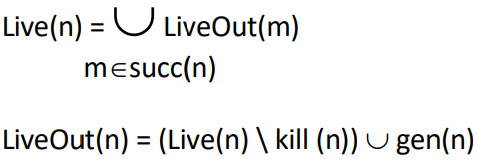
\includegraphics[width=0.4\textwidth,keepaspectratio]{live_exp}
    \end{figure}
\end{enumerate}

\textblue{Classification of analyses} :
\begin{itemize}
    \item \textblue{Forward/backward} : a node’s set depends on that of its predecessors/successors
    \item \textblue{Any-path/all‐path} : a node’s set contains a value iff it is coming from any/all of its inputs
\end{itemize}

\begin{figure}[H]
    \centering
    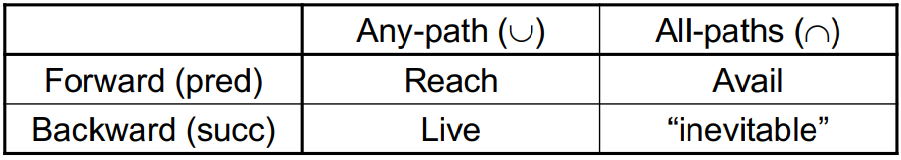
\includegraphics[width=0.5\textwidth,keepaspectratio]{classification_of_analyses}
\end{figure}

\section{Discuss the effect of pointers and procedures.}

\begin{enumerate}
    \item \textblue{Arrays and pointers} : introduce \textblue{uncertainty} : do different expressions access the same storage ?
    
    For example: $a[i]$ is the same as $a[k]$ when $i=k$ or $a[i]$ same as $b[i]$ when $a=b$. 
    
    \textblue{Solution}: 
    \begin{enumerate}
        \item \textblue{Any-path} : Gen sets contains all potential aliases, kill sets contain only what is definitely modified.
        \item \textblue{All-path} : Gen sets contains only the defined variables, kill sets contain the what is definitely modified and the potential aliases
    \end{enumerate}
    \item \textblue{Procedures} : \textblue{interprocedural} (Across several methods or procedures) data flow analysis has critical and difficult cost/precision trade-offs: context sensitivity and flow sensitivity.
    
    For example: Reach, Avail,... are flow-sensitive and \textblue{intraprocedural} (Within a single method or procedure) analyses which cost \bigO$(n^3)$ for one procedure (reasonably cheap) but what about doing flow-sensitive interprocedural analyses? $\rightarrow$ \bigO$(n^3)$ on the whole program : prohibitive ! So, many interprocedural flow analyses are flow-insensitive (it is often good enough, e.g. type checking)
\end{enumerate}

\chapter{Functional testing}

\section{Define test case, test obligation, adequacy criterion, test satisfaction}

\begin{enumerate}
    \item \textblue{Test case} : A set of inputs, execution conditions, and a pass/fail criterion for judging test execution
    \item \textblue{Test case specification} : A requirement to be satisfied by one or more test cases
    \item \textblue{Test obligation} : A partial test case specification, requiring some property deemed (= considered) important to thorough testing
    \item \textblue{Adequacy criterion}: A predicate that a <program, test suite> pair must satisfy to be adequate; usually expressed in the form of a rule for deriving a set of test obligations from another artefact (program, specification)
    \item \textblue{Test satisfaction}:
    A test suite (set of test cases) satisfies an adequacy criterion if :
    \begin{itemize}
        \item All the tests succeed (pass)
        \item Every obligation is satisfied by at least one test case
    \end{itemize}
\end{enumerate}

\textblue{Infeasible Criterion}: Sometimes no test suite can satisfy a criterion for a given program
\begin{itemize}
    \item [$\Rightarrow$] Solution : eliminate infeasible test obligations\\
    $\hookrightarrow$ Undecidable in the general case
    \item [$\Rightarrow$] \textblue{Solution}: measure fraction of obligations covered\\
    $\hookrightarrow$ Coverage = \% of obligations covered
\end{itemize}

\section{Define functional and structural testing}

\begin{enumerate}
    \item \textblue{Functional testing} : (black box, closed box)
    \begin{itemize}
        \item Program content is unknown or ignored
        \item Test input/output behaviour
        \item Obligations from functional specifications (informal textual specs, tables, state graphs, UML, ...)
        \item [$\hookrightarrow$] Functional testing is \textblue{systematic testing} (select inputs that are especially valuable, different classes, limit cases, special values)
    \end{itemize}
    \item \textblue{Structural testing} : (white box, clear box)
    \begin{itemize}
         \item Program content is visible and observed (e.g. if test suite executes all program statements/conditions/branches/..., then coverage is 100\%)
         \item Test internal operation
         \item Obligations from program code
     \end{itemize}
\end{enumerate}

\newpage
\section{Explain category-partition testing}

\textblue{Category-partition testing} : 3 steps
\begin{enumerate}
    \item \textblue{Decompose the specification into units, parameters, categories}
    \begin{enumerate}
        \item Identify independently testable units
        \item For each unit, identify parameters and environment elements
        \item For each parameter, identify categories (characteristics) $\rightarrow$ Not a trivial task ! No hard-and-fast rules, reflect test designer’s judgment,...
    \end{enumerate}
    \item \textblue{Identify relevant choices (values) for each category}
    \begin{enumerate}
        \item Identify classes of values for each category (ignore interactions
between different categories)

        \item Boundary value testing
        \begin{enumerate}
            \item extreme values within a class
            \item values just outside the class
            \item interior (non-extreme) values
        \end{enumerate}
        \item Erroneous condition testing : values outside the normal domain of the program
    \end{enumerate}
    \item  \textblue{Introduce constraints} : combination of values for each category corresponds to a test case specification. Number of combinations = product of category sizes, most of which are impossible ! Introduce constraints to rule out impossible combinations, or to reduce the size of the test suite if too large
\end{enumerate}

\section{Explain pairwise and n-wise testing}

Category-partition testing is a systematic approach to generate combinations, but the test suite size grows very rapidly with the number of categories (even with constraints). The idea of pairwise testing is to use a non-exhaustive approach

\begin{enumerate}
    \item \textblue{Pair-wise testing} : all \textblue{pairs of choices}
    \begin{itemize}
        \item \textblue{Pairwise combination} : generate combinations that efficiently cover all pairs (triples,... in case of n-wise) of choices. Justified by the fact that most failures are triggered by a single value or a combination of a few values, so covering pairs (triples,...) reduces the number of test cases, but reveals most faults
        \item \textblue{Complexity} : For N categories with M choices each :
        \begin{itemize}
            \item \textblue{All combinations} $=$ \bigO$(M^N)$ test cases $\rightarrow$ exponential in number of categories
            \item \textblue{All pairs} $=$ \bigO$(M^2  log(N))$ test cases $\rightarrow$ logarithmic in number of categories
        \end{itemize}
    \end{itemize}
    \item \textblue{N-wise testing} : Same as pairwise but for all N-tuples of choices
\end{enumerate}

\newpage
\section{Explain catalog-based testing}

\begin{itemize}
    \item Deriving value classes requires human judgment, catalog-based testing aims to gather experience in a systematic collection
    \item Catalogs list important cases for each possible type of variable
\end{itemize}

\textblue{Benefits} :
\begin{itemize}
    \item Speed up the test design process
    \item Routinise many decisions, better focusing human effort
    \item Accelerate training and reduce human error
\end{itemize}

\textblue{Process} :
\begin{enumerate}
    \item Analyse the initial specification to identify simple
elements : pre-conditions, post-conditions, definitions,
variables, operations
    \item Derive a first set of test case specifications from pre-conditions, post-conditions
and definitions
    \item Complete the set of test case specifications using test catalogs
\end{enumerate}


\textblue{Catalog} :

\begin{itemize}
    \item Each entry $=$ a kind of element that can occur in a specification
    \item Each entry is associated with a list of generic test case specifications
\end{itemize}

\textblue{Example} :

\begin{itemize}
    \item Catalog entry Boolean
    \item Two test case specifications : $true, false$
    \item Label in/out indicate if applicable only to $input/output$ or $both$
\end{itemize}

\begin{figure}[H]
    \centering
    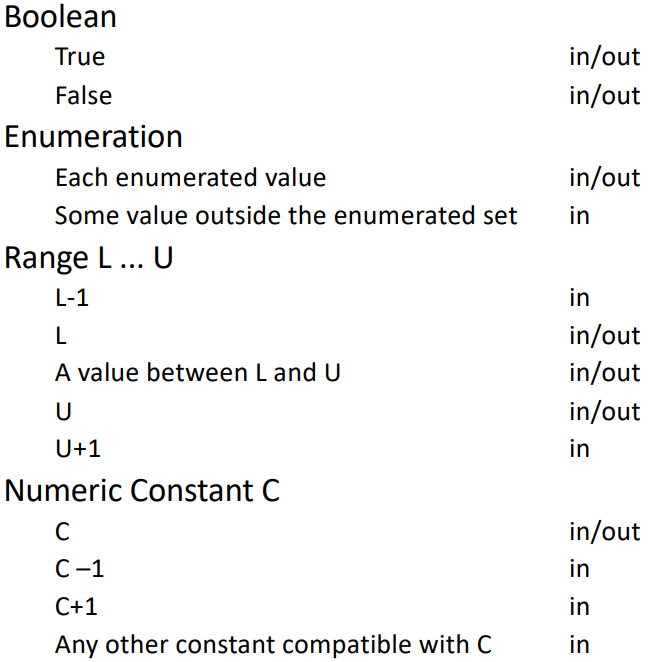
\includegraphics[width=0.5\textwidth,keepaspectratio]{catalog_ex}
\end{figure}

\chapter{Structural testing}

\section{Define statement, branch and condition coverage, compound conditions and MC/DC, and compare their strengths}

\begin{enumerate}
    \item \textblue{Statement coverage}\\
    Each statement must be executed at least once.\\
    Motivation : a fault in a statement can only be revealed by executing the faulty statement 
    $$C_{stmt} = \frac{\#executed\ statement}{\#statement}$$
    NB : CFG nodes $\neq$ statements : may represent basic blocks, multiple statements or parts of statements. Difference in granularity, not in concept (100\% node coverage = 100\% statement coverage)
    \item \textblue{Branch coverage}\\
    Each branch must be executed at least once.\\
    Variant: edge coverage → each edge in the CFG.\\
    In a graph: traversing all edges $\Rightarrow$ visiting all nodes.
    $$C_{branch} = \frac{\#executed\;branches}{\#branches}$$
    NB: 100\% branch coverage $\Rightarrow$ 100\% statement coverage\\
    Branch coverage = \textblue{decision coverage} : each decision must be true and false at least once (decision = top-level boolean expression)
    \item \textblue{Condition coverage}\\ 
    Considers case analysis in more detail : individual conditions in a boolean decision are tested. Each \textblue{basic condition} must be true and false at least once.
$$C_{bcond} = \frac{
\begin{gathered}
\#executed\;true\;basic\;conds\\
+\#executed\;false\;basic\;conds
\end{gathered}
}{2*\#basic\;conds}$$
    Note: basic condition coverage can be satisfied without satisfying branch coverage. Branch and basic condition are not comparable $\rightarrow$ neither implies the other
    \item \textblue{Compound conditions coverage}\\ 
    Each possible evaluation of each decision must be taken at least once: all branches of the decision tree.\\
    Note : exponential complexity. $N$ conditions $\Rightarrow$ \bigO$(2^N)$ test cases
    \begin{figure}[H]
        \centering
        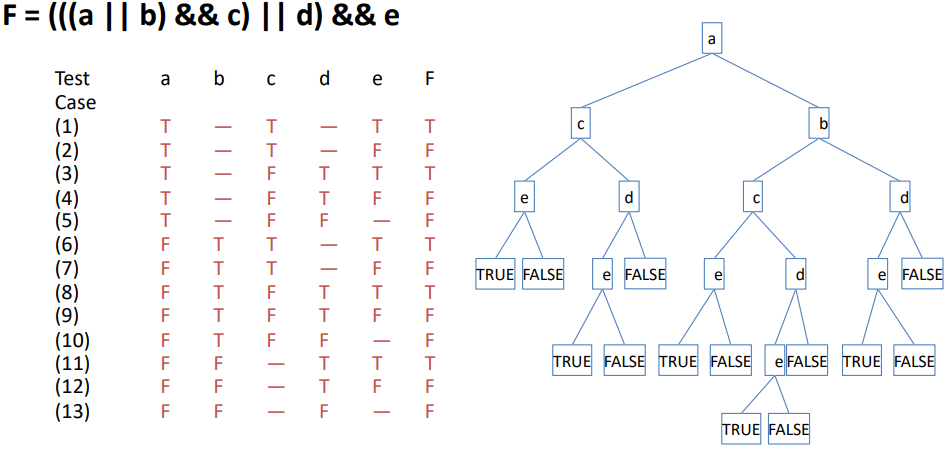
\includegraphics[width=0.9\textwidth,keepaspectratio]{exp_compl}
    \end{figure}
    \item \textblue{MC/DC (Modified condition/decision) coverage}
    
    \begin{minipage}{0.7\textwidth}
        Each basic condition is shown to independently affect the decision\\
        Motivation : test important combinations of conditions, without exponential blow-up\\
        Requires, for each basic condition $C$ in a decision $D$, two test cases such that:
        \begin{enumerate}
            \item Values of all evaluated conditions except $C$ are the same and 
            \item $D$ evaluates to true for one and false for the other
        \end{enumerate}
    \end{minipage}
    \hfill
    \begin{minipage}{0.22\textwidth}
    \begin{figure}[H]
        \centering
        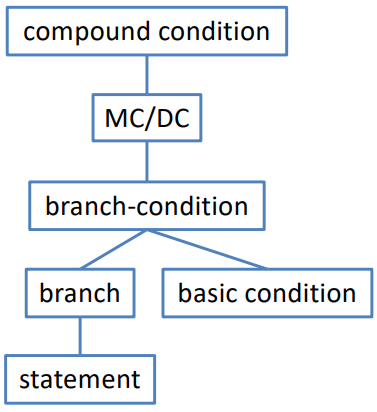
\includegraphics[width=\textwidth,keepaspectratio]{mc_dc_1}
    \end{figure}
    \end{minipage}
    N basic conditions $\Rightarrow$ N+1 test cases (linear complexity)
    \begin{figure}[H]
        \centering
        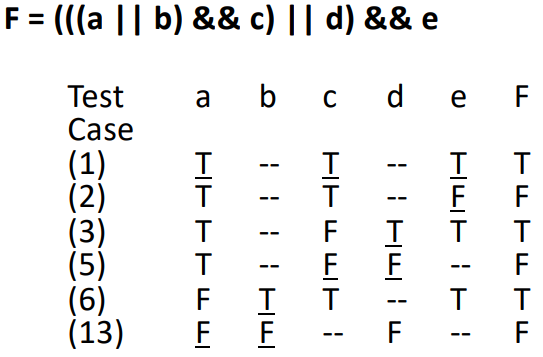
\includegraphics[width=0.35\textwidth,keepaspectratio]{mc_dc_2}
    \end{figure}
    It is a good balance of thoroughness and test size (and therefore widely used).

    It is basic condition coverage ($C$) + decision (=branch) coverage ($DC$) + one additional condition ($M$) that every condition must independently affect the decision’s output.
\end{enumerate}

\section{Define path coverage, discuss limitations and show some practical path coverage criteria}

\begin{itemize}
    \item \textblue{Path coverage} : decision and condition coverage only consider individual program decisions. Many more paths than branches. Each path must be executed at least once
    $$C_{path} = \frac{\#executed\ paths}{\#paths}$$
    \item \textblue{Limitations} :
    \begin{enumerate}
        \item Program with loops $\Rightarrow$ infinite number of paths ! Full path coverage is therefore usually impossible to satisfy.
        \item Feasible criterion : partition infinite set of paths into a finite number of classes, by limiting :
        \begin{enumerate}
            \item the number of traversals of loops
            \item the length of the paths to be traversed
            \item the dependencies among selected paths
        \end{enumerate}
    \end{enumerate}
    \item \textblue{Some practical path coverage criteria} :
    \begin{itemize}
        \item \textblue{Boundary interior path coverage} : each path up to the first repeated node must be executed at least once
        \begin{enumerate}
            \item Group together paths that differ only in the subpath they follow when repeating the body of a loop
            \item Construction: unfold the CFG up to the first repeated node
            \item Limitations: the number of paths can still grow exponentially
        \end{enumerate}
        \item \textblue{Cyclomatic coverage}: a basis of independent paths must be executed
        \item \textblue{Loop boundary coverage}: each loop body must be iterated zero times, one time and more than one time at least once.
    \end{itemize}
\end{itemize}

\section{Define data flow coverage criteria}

\begin{enumerate}
    \item \textblue{All DU (def-use) pairs}: \textit{each DU pair} is exercised \textit{at least once}
    \item \textblue{All DU paths} : \textit{each simple (non looping) DU path} is exercised \textit{at least once} (often impractical)
    \item \textblue{All definitions}: \textit{for each definition, some DU pair} is exercised \textit{at least once} (every computed value is used somewhere)
\end{enumerate}

\section{Discuss the problems of aliases and infeasibility}

\begin{itemize}
    \item \textblue{Problem with aliases} : which references are (always or sometimes) the same ?\\
    Ex: $p=\&x; ...; *p=99 \rightarrow *p$ is an alias of $x$
    \item \textblue{Problem of infeasibility}: with conditional statement, it is possible that a variable is defined and never used = infeasibility problem. This problem is relevant, combinations of elements matter, it is impossible to decide feasible paths. In practice, we achieve reasonable coverage, but full coverage is usually unattainable. Number of paths is exponential in worst case, but often linear. But testing all DU paths is more often impractical since attainability is an undecidable problem
\end{itemize}

\chapter{Model-based testing}

\section{Explain the principles of model-based testing}

\begin{enumerate}
    \item It is used in order to test structured specifications (state machines, tables, graphs, grammars,...)
    \item Consist on devising test cases to check actual behaviour against behaviour specified by the model
    \item Coverage similar to structural testing, but applied to specification and design model
\end{enumerate}

\section{Explain path-insensitive and path-sensitive state machine coverage criteria}

\begin{enumerate}
    \item \textblue{Covering finite state machine} :\\
    Finite state machines: for describing behaviour that depends on sequences of events or stimuli
    \begin{itemize}
        \item \textblue{State coverage} : every state in the model should be visited at least once
        \item \textblue{Transition coverage} : every transition in the model should be traversed at least once (this is the most commonly used criterion).\\
        Transition coverage assumes that \textblue{transitions depend only on current state} and not on path to reach the state. This is not always true $\rightarrow$ needs path-sensitive criteria
    \end{itemize}
    \item \textblue{Path-sensitive criteria} :
    \begin{itemize}
        \item \textblue{Single state path coverage}: traverse each subpath that reached states at most once
        \item \textblue{Single transition path coverage}: traverse each subpath that reaches transitions at most once
        \item \textblue{Boundary interior loop coverage}: traverse each distinct loop the minimum, an intermediate, and the maximum or a large number of times (the most common)
    \end{itemize}
\end{enumerate}

\section{Discuss coverage criteria for decision structures and grammars}

\begin{itemize}
        \item \textblue{Coverage criteria for decision structures} :\\
        A representation of a function $result = F(conditions)$\\
        $n$ conditions $\rightarrow$ $2^n$ possible combinations (decision tables/trees, flow charts).\\
        Treat as \textblue{Boolean expressions}.\\
        \textblue{Covering} : Apply condition / decision‐based criteria : 
        \begin{enumerate}
            \item \textblue{Basic condition coverage} : a test case for each column
            \item \textblue{Compound condition coverage} : a test case for each (possible) combination of basic conditions
            \item \textblue{Modified coverage (MC/DC)} : add columns that differ in one input row and in outcome, merge compatible columns, a test case specification for each column
        \end{enumerate}
        
        \item \textblue{Coverage criteria for decision grammars} : \\
        Useful for sequences and nested structure. Test cases are string generated from the grammar : 
        \begin{enumerate}
            \item \textblue{Production coverage} : each production must be used at least once
            \item \textblue{Boundary condition coverage} : each recursive production must be used ($min$, $min+1$, $max-1$, $max$) times, where min and max are set for each production (similar to boundary interior path)
        \end{enumerate}
        Test cases generated depend on generation strategy:
        \begin{enumerate}
            \item Productions with non-terminals first $\rightarrow$ few, large test cases
            \item Productions with terminals first $\rightarrow$ many, small test cases
        \end{enumerate}
\end{itemize}

\chapter{Object-oriented testing}

\section{Explain the principles of testing of object-oriented software, at the unit and integration level}

For an object oriented software : \textblue{unit} = single class (or cluster of strongly related classes e.g. exceptions)
\begin{itemize}
    \item [$\Rightarrow$] \textblue{Unit testing} = \textit{intra}-class testing
    \item [$\Rightarrow$] \textblue{Integration testing} = \textit{inter}-class testing
\end{itemize}

\section{Discuss structural coverage criteria for intra- and inter-class testing}

\begin{minipage}[t]{0.48\textwidth}
    \textblue{Inter-class testing} (state machine):
    \begin{itemize}
        \item Test interactions between classes
        \item Bottom-up integration, according to\\ "depends" relation
        \item Use / include hierarchy:
        \begin{enumerate}
            \item $A$ uses $B = A$ makes method calls on $B$
            \item $A$ includes $B = A$ objects include references to $B$ objects, ignore inheritance, abstract classes
        \end{enumerate}
        \item Bottom-up integration, clustering
    \end{itemize}
\end{minipage}
\hfill
\begin{minipage}[t]{0.48\textwidth}
    \textblue{Intra-class testing} :
    Basic idea :
    \begin{itemize}
        \item Objects have a state
        \item Methods calls are state transitions
        \item Test cases are sequences of method calls
    \end{itemize}
    State machine can be derived from specification and code $\rightarrow$ Model-based testing, state / transition coverage
\end{minipage}
   
\begin{minipage}[t]{0.48\textwidth} 
    \textblue{Inter-class structural testing} :\\
    DU pair structural testing:
    \begin{itemize}
        \item Working bottom-up in dependence hierarchy (leaf classes, then classes that use leaf classes, ...)
        \item Classify each method:
        \begin{enumerate}
            \item \textblue{Inspectors} : use, but do not modify, object state
            \item \textblue{Modifiers} : modify, but not use, object state
            \item \textblue{Inspector / modifiers} : use and modify object state
            \item Treating a whole object as variable (not each field)
        \end{enumerate}
        \item Treat inspector calls as uses, modifier calls as defs
    \end{itemize}
\end{minipage}
\hfill
\begin{minipage}[t]{0.48\textwidth}
    \textblue{Intra-class structural testing} :
    \begin{itemize}
        \item As for procedural software, start with functional testing (from specifications), then complete with structural testing (from the code)
        \item Use control flow graph :\\
        Each method $+$\\
        Node for class $+$\\
        Edges $\rightarrow$ method, method $\rightarrow$ class\\
        $\Rightarrow$ control flow through sequences of method calls
    \end{itemize}
\end{minipage}

\begin{figure}[H]
    \centering
    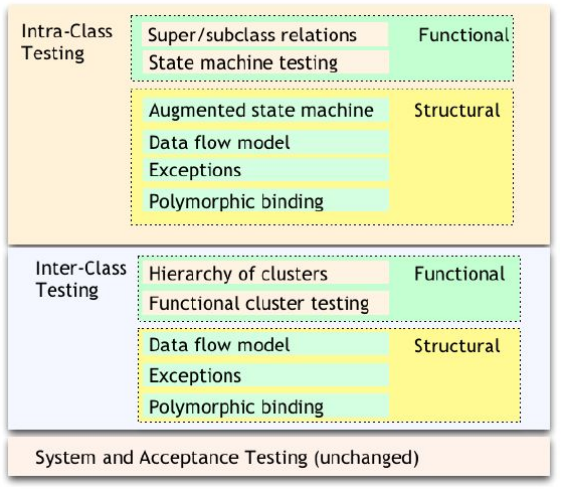
\includegraphics[width=0.5\textwidth,keepaspectratio]{intra_inter_class_testing}
\end{figure}

\section{Discuss the issues of test oracles, polymorphism and exception handling}

\begin{enumerate}
    \item \textblue{Test oracles} must be able to check the correctness of a test execution
    \begin{itemize}
        \item \textblue{Correct output} : OK, can be checked
        \item \textblue{Correct new state} : not accessible, encapsulation
    \end{itemize}
    Accessing the state:
    \begin{itemize}
        \item \textblue{Intrusive approach} : use language constructs, add inspector methods → breaks encapsulation, may produce undesired results
        \item \textblue{Equivalent scenarios approach} : generate equivalent sequences of method calls, compare the final states of the objects
    \end{itemize}
    \item \textblue{Polymorphism} : Combinatorial explosion problem (dynamic bindings). When testing a child class, we would like to test only what is needed not what has been tested in the parent class (any method whose behaviour has been changed)\\
Testing history approach : 
\begin{enumerate}
    \item Track test suites and test executions
    \begin{itemize}
        \item Determine which new tests are needed
        \item Determine which old tests must be re-executed
    \end{itemize}
    \item New and changed behaviour
    \begin{itemize}
        \item New methods must be tested
        \item Redefined methods must be tested, we can partially reuse test suites
        \item Unchanged methods need not be retested
    \end{itemize}
    \item Executing test cases is usually cheap, it may be simpler to re-execute the full parent test suite
\end{enumerate}

    \item \textblue{Exceptions} : 
    \begin{enumerate}
        \item \textblue{Exceptions} 
        \begin{itemize}
            \item Implicit control flows
            \item May be handled by different handler
        \end{itemize}
        Impractical to treat exceptions like normal flow
        \begin{itemize}
            \item Too many flows: every exception source times every exception handler
        \end{itemize}
        \item \textblue{Program error exceptions} : test to prevent them, not to handle them.
        \item \textblue{Explicit throws} : test with respect to every handler on call stack
        \item \textblue{Local exception handlers} : test the exception handler
        \item \textblue{Non-local exception handlers} :
        \begin{itemize}
            \item Difficult to determine all <source, handler> pairs
            \item Design rule: if a method propagates an exception, the method call should have no other effect
            \item Test all sources, all handlers (but not all pairs)
        \end{itemize}
    \end{enumerate}
\end{enumerate}

\chapter{Fault-based testing}

\section{Explain the principles and assumptions of mutation testing}

\begin{itemize}
    \item \textblue{Principles} :
    \begin{enumerate}
        \item A mutation is a syntactic change (a seeded fault) $\rightarrow$ ex: change ($i<0$) to ($i\leq0$)
        \item A mutant is a copy of a program with a mutation (valid mutant = syntactically correct)
        \item Run test suite on all the mutants
        \item A mutant is killed if it fails on at least one test case
        \item If many mutants are killed then the test suite is effective at finding real faults
    \end{enumerate}
    \item \textblue{Assumptions} :
    \begin{enumerate}
        \item \textblue{Competent programmer hypothesis} :\\
        Programs are assumed to be nearly correct. Real faults are small variations from correct program. Mutants are reasonable models of real faults
        \item \textblue{Coupling effect hypothesis} : \\
        Tests that find simple faults also find more complex faults. Even if mutants are only simple faults, a test suite that kills mutants is good at finding complex faults too
    \end{enumerate}
\end{itemize}

\section{Give examples of mutation operators}

\begin{enumerate}
    \item \textblue{crp}: constant for constant replacement : $(x < 5) \rightarrow (x < 12)$
    \item \textblue{ror}: relational operator replacement : $(x \leq 5) \rightarrow (x < 5)$
    \item \textblue{vie}: variable initialization elimination : $int\ x = 5; \rightarrow int\ x;$
\end{enumerate}

\section{Discuss fault-based coverage measures}

There are two possible reasons that a mutant survive:
\begin{enumerate}
    \item \textblue{The mutant is equivalent to the original program}. The mutation does not change the behaviour. The seeded fault is not really a fault.
    \item \textblue{The test suite is inadequate}. The mutant could have been killed, but was not. Adding a test case for just this mutant is a bad idea : we care about the real bugs, not the fakes.
\end{enumerate}

\noindent \textblue{Fault-based coverage} : All non-equivalent mutants are killed by at least one test case
$$C_{Fault} = \frac{\#killed\;mutant}{\#non-equiv\ mutant}$$

\section{Discuss ways to reduce the cost of mutation testing}

Equivalent mutants are hard to determine (undecidable in the worst case) and there are lots of mutants
\begin{itemize}
    \item[$\hookrightarrow$] High cost; Grows with the square of program size; Running each test case on each mutant is expensive
\end{itemize}

\textblue{Solutions} : 
\begin{enumerate}
    \item \textblue{Weak mutation} : observe states of program and mutant, kill as soon as a difference is found (do not wait for test completion)
    \item \textblue{Meta-mutant} : mutant with several seeded faults, with mechanism to activate the mutants (check several mutants in one test run)
    \item \textblue{Statistical mutation} : create a random sample of mutants (OK for assessing a test suite)
\end{enumerate}

\section{Explain fault estimation using seeded faults or independent test groups}

\begin{enumerate}
    \item\textblue{Seeded faults} :\\
    How many remaining (natural) faults $N$ ?\\
    Intentionally seed $S$ faults in the program\\
    Run the tests
    \begin{itemize}
        \item $s$ discovered seeded faults
        \item $n$ discovered natural faults
    \end{itemize}
    \textblue{Hypothesis}: same effectiveness $\frac{n}{N} = \frac{s}{S}$
    \begin{itemize}
        \item [$\Rightarrow$]$N = \frac{S * n}{s}$
    \end{itemize}

    \item \textblue{Independent test groups} :\\
    If we don’t know typical faults ?\\
    Split tests in two groups $E_1$, $E_2$
    \begin{itemize}
        \item $n_1$ faults detected by $E_1$
        \item $n_2$ faults detected by $E_2$
        \item $n_{12}$ faults detected by both $E_1$ and $E_2$
        \item $N$ faults in total
    \end{itemize}

    \textblue{Hypothesis} : effectiveness of $E_1$ is the same on all faults as on faults detected by $E_2$:
    \begin{itemize}
        \item [$\Rightarrow$]$\frac{n_1}{N} = \frac{n_{12}}{n_2}$
        \item [$\Leftrightarrow$]$N = \frac{n_1 * n_2}{n_{12}}$
    \end{itemize}
\end{enumerate}

\begin{figure}[H]
    \centering
    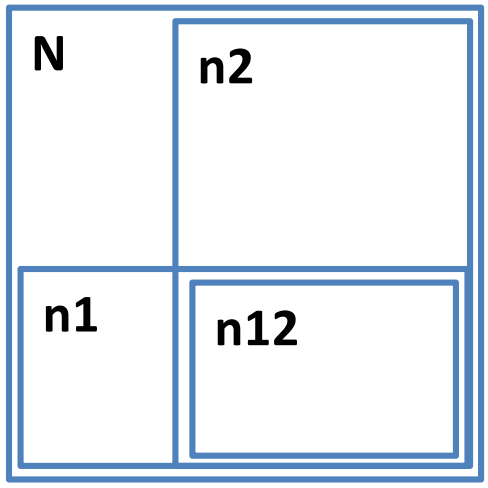
\includegraphics[width=0.2\textwidth,keepaspectratio]{fault_estimation}
\end{figure}

\chapter{Test execution I}

\section{Describe the principles of scaffolding for test execution}

\textblue{Scaffolding} (échafaud) : code produced to support development activities especially testing. Not part of the product. May be temporary.

\begin{minipage}{0.74\textwidth}
    It includes :
    \begin{enumerate}
        \item \textblue{Test harness} : environment in which the component is tested. Ex: Software simulation of a hardware device
        \item \textblue{Test driver} : calls the component. Applies the test cases. A "main" program for running a test
        \item \textblue{Test stubs} : called by the component. Substitutes for called components
    \end{enumerate}
\end{minipage}
\hfill
\begin{minipage}{0.25\textwidth}
    \begin{figure}[H]
        \centering
        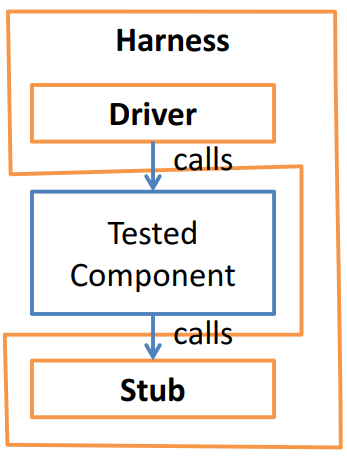
\includegraphics[width=0.55\textwidth,keepaspectratio]{scaffolding_1}
    \end{figure}
\end{minipage}

\begin{minipage}{0.74\textwidth}
    The scaffolding must provide : 
    \begin{enumerate}
        \item \textblue{Controllability} : allow to execute test cases
        \item \textblue{Observability} : allow to judge the outcome of tests
        \item [$\Rightarrow$] May require additional interfaces, drivers
    \end{enumerate}
\end{minipage}
\hfill
\begin{minipage}{0.25\textwidth}
    \begin{figure}[H]
        \centering
        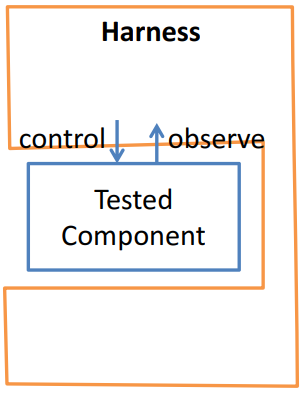
\includegraphics[width=0.55\textwidth,keepaspectratio]{scaffolding_2}
    \end{figure}
\end{minipage}

\begin{figure}[H]
    \centering
    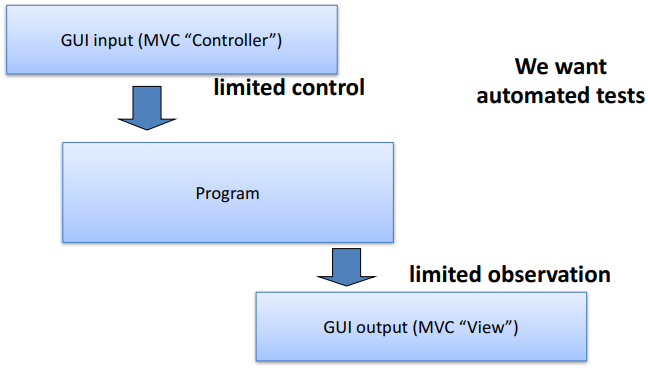
\includegraphics[width=0.49\textwidth,keepaspectratio]{scaffolding_3}\hfill
    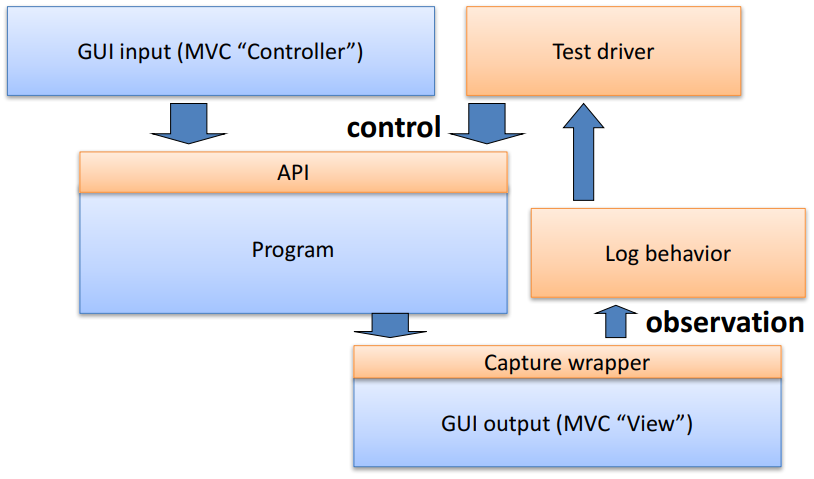
\includegraphics[width=0.49\textwidth,keepaspectratio]{scaffolding_4}\hfill
    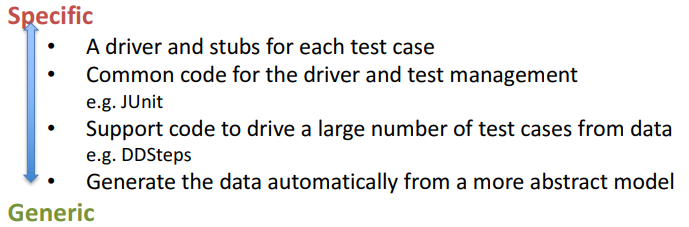
\includegraphics[width=0.49\textwidth,keepaspectratio]{scaffolding_5}
\end{figure}

\newpage
\section{Discuss different types of test oracles}

Did this test case succeed, or fail ? \textblue{Oracle} : software that determines whether a test passed or failed.

Better than manual checking :
\begin{enumerate}
    \item More efficient
    \item More reliable
    \item More capable (e.g timing, large data)
\end{enumerate}
Oracles should ideally :
\begin{itemize}
    \item Report \textgreen{PASS} for \textblue{all} \textgreen{correct} executions
    \item Report \textred{FAIL} for \textblue{all} \textred{incorrect} executions
\end{itemize}

\textblue{Partial oracles} :
\begin{itemize}
    \item Must report PASS for \textgreen{all correct} executions
    \item May report PASS for \textred{some incorrect} executions
\end{itemize}
No false alarms (\textred{FAIL} on correct executions). Several partial oracles may be more effective than one complete oracle.
    
\textblue{Comparison‐Based Oracle} :

\begin{minipage}{0.58\textwidth}
    Oracle compares actual to expected output, reports if (actual = expected) then \textgreen{PASS} else \textred{FAIL}. Fine for a small number of hand‐generated test cases (e.g. JUnit test cases: assertEquals(actual, expected)).
\end{minipage}
\hfill
\begin{minipage}{0.40\textwidth}
    \begin{figure}[H]
        \centering
        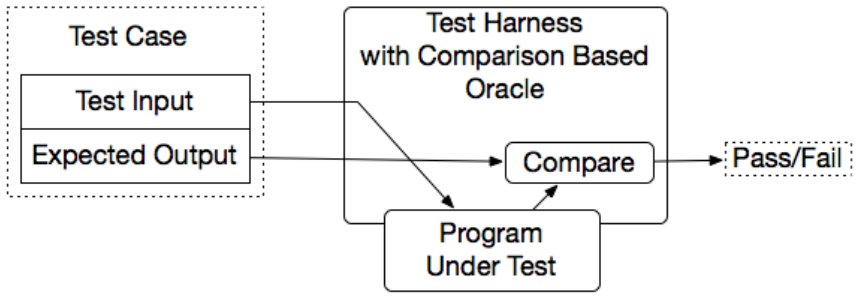
\includegraphics[width=\textwidth,keepaspectratio]{comparison_based_oracle}
    \end{figure}
\end{minipage}
   
\textblue{Self‐Checks as Oracle} :

\begin{minipage}{0.58\textwidth}
    \begin{itemize}
        \item [$\oplus$]Usable with large, automatically generated test suites
        \item [$\ominus$]Often only a partial check (e.g., structural invariants of data structures)
    \end{itemize}
\end{minipage}
\hfill
\begin{minipage}{0.40\textwidth}
    \begin{figure}[H]
        \centering
        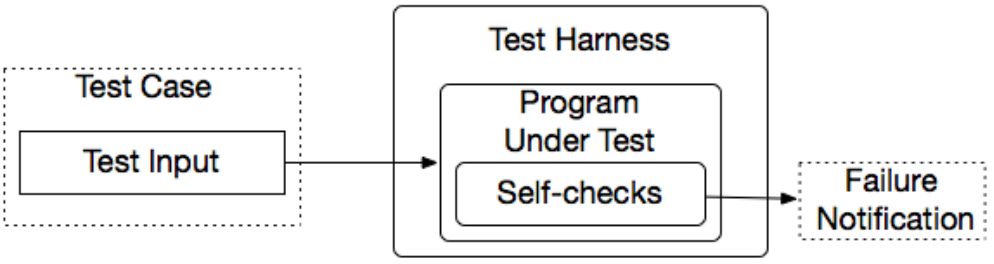
\includegraphics[width=\textwidth,keepaspectratio]{self_checks_oracle}
    \end{figure}
\end{minipage}
    
\textblue{Assertions as Oracle} :
\begin{itemize}
    \item \textblue{Invariants on data structures} (e.g. "assert 0 <= size \&\& size <= a.length")
    \item \textblue{Pre‐ and post‐conditions} (e.g. "assert k != null; v = dict.get(k); assert dict.contains(k, v);")
\end{itemize}
May need to deal with quantifiers. implement as iteration $\Rightarrow$ does not scale well or sample some elements (partition testing)
    
\textblue{Capture and Replay} :
\begin{itemize}
    \item \textblue{Capture} a manually run test case, sequence of inputs, outputs
    \item \textblue{Replay} it automatically with a comparison‐based oracle and compare actual to captured outputs
\end{itemize}
\begin{figure}[H]
    \centering
    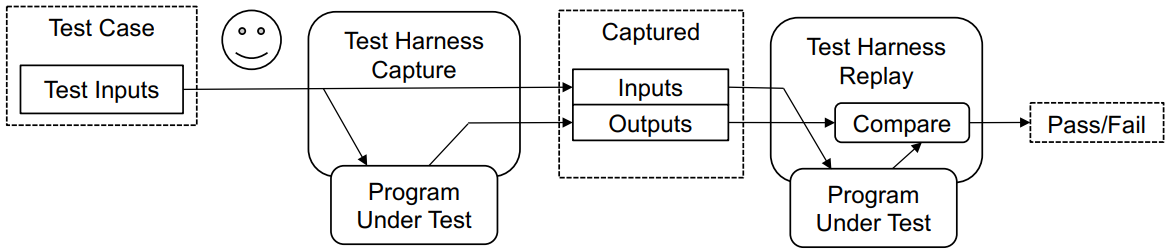
\includegraphics[width=0.5\textwidth,keepaspectratio]{capture_replay_oracle}
\end{figure}

Reusable only until a program change invalidates it. Lifetime depends on abstraction level of input and output.

\section{Describe the nature and objectives of unit and integration testing activities}

\begin{figure}[H]
    \centering
    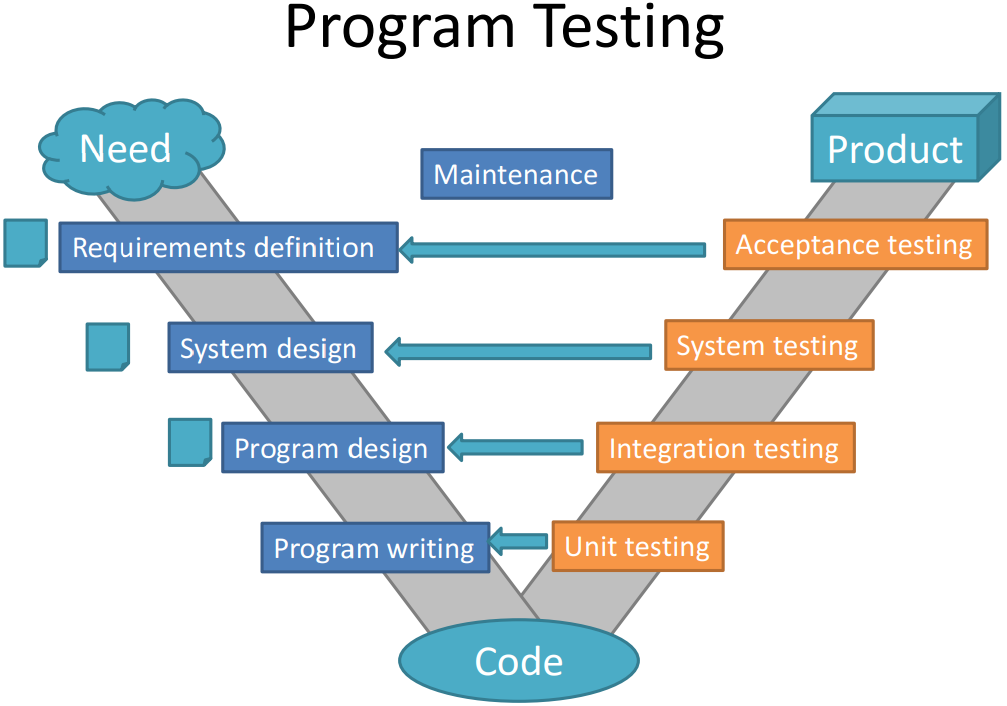
\includegraphics[width=0.49\textwidth,keepaspectratio]{program_testing}\hfill
    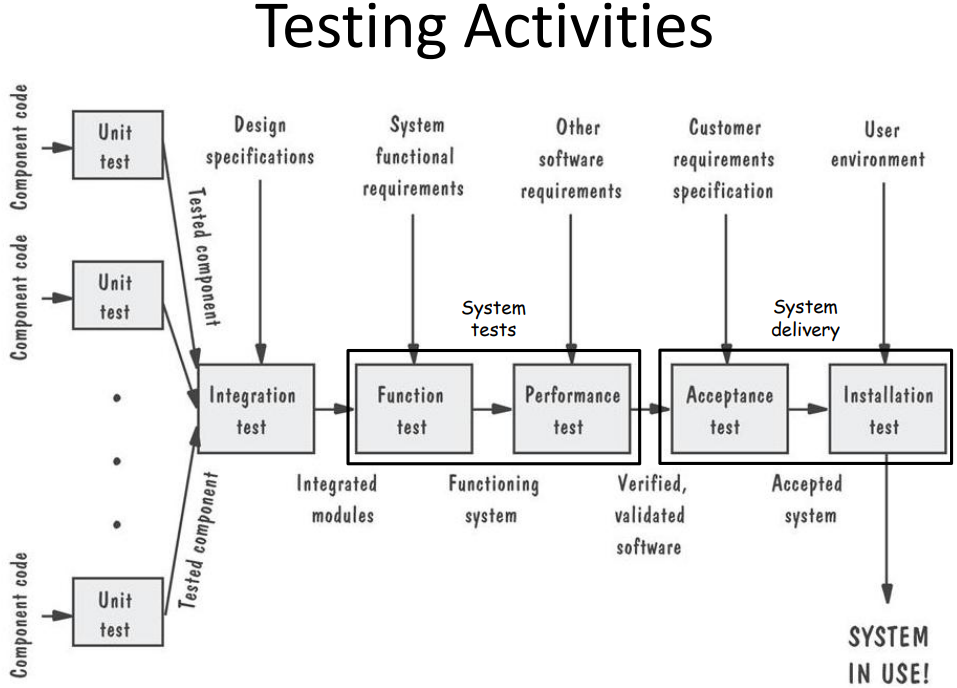
\includegraphics[width=0.49\textwidth,keepaspectratio]{testing_activities}
\end{figure}

\begin{itemize}
    \item \textblue{Unit Testing} : Aka module testing, component testing
    \begin{itemize}
        \item Testing : feed inputs, check valid outputs
        \item Code reviews, analysis : check internal data structures, logic 
    \end{itemize}
    \item \textblue{Integration Testing} : 
    \begin{itemize}
        \item Assemble components together
        \item Check correct interaction
    \end{itemize}
\end{itemize}

\section{Discuss and compare different integration testing strategies}

\begin{figure}[H]
    \centering
    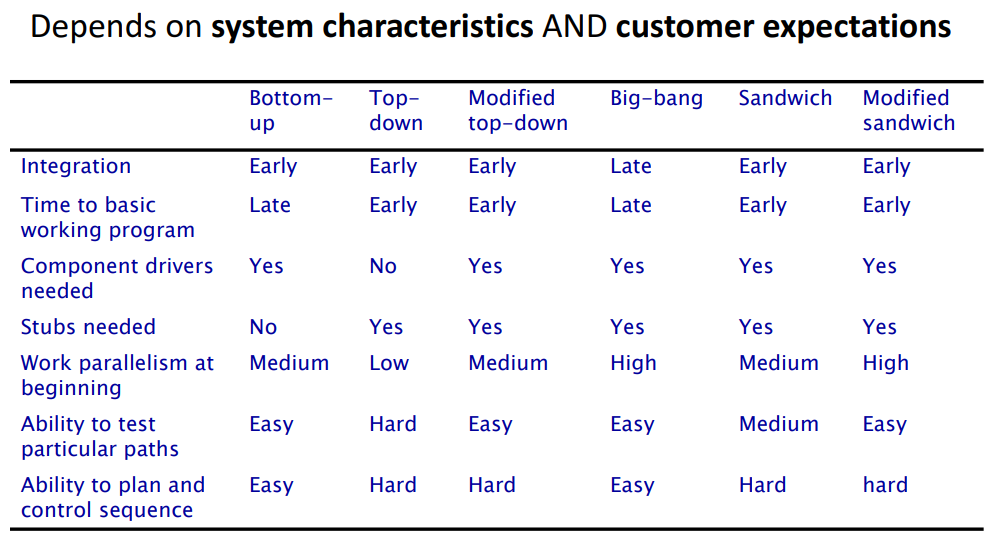
\includegraphics[width=0.8\textwidth,keepaspectratio]{str_int_strategies}
\end{figure}

\textblue{Functional integration strategies} :
\begin{itemize}
    \item \textblue{Threads} :\\
    \textit{Thread} = user-visible program feature across several modules (e.g. send a messages, change user, create mailbox, ...)\\
    Test each thread incrementally.\\
    $\Rightarrow$ Minimizes stubs and drivers but integration plan may be complex
    \item \textblue{Critical modules} :\\
    Test modules with highest risk first and integrate them with thread or sandwich strategy.\\
    $\Rightarrow$ Requires risk assessment first.
\end{itemize}

\chapter{Test execution II}

\section{Describe the nature and objectives of system, acceptance and regression testing activities}

\begin{figure}[H]
    \centering
    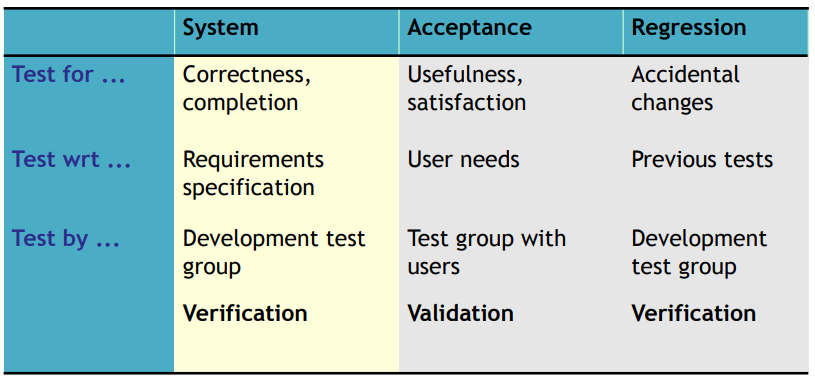
\includegraphics[width=0.7\textwidth,keepaspectratio]{testing_comparison}
\end{figure}

\begin{itemize}
    \item \textblue{System Testing}
    \begin{itemize}
        \item Based	on a requirements specification of observable behaviour
        \begin{itemize}
            \item Functional and non-functional (performance)
            \item Not user needs (validation), not opinion
        \end{itemize}
        \item Independent of design	and	implementation (avoid repeating software design errors	 in system test design)
    \end{itemize}
    \item \textblue{Acceptance Testing}
    \begin{itemize}
        \item Goal : enable the customers and users to determine if the system meets their needs (uncover remaining requirement discrepancies and needs unspecified in the requirements)
        \item Measuring	quality, not searching for faults (fundamentally different goal than system testing)
    \end{itemize}
    \item \textblue{Regression Testing}
    \begin{itemize}
        \item Regression = loss of correct functionality after a change (adding new features; changing, adapting conditions; bugs fixing)
        \item \textblue{Regression testing} $=$ re‐executing tests after any change to detect regressions
        \item Can be a major cost of software maintenance. Sometimes much more than making the change
    \end{itemize}
\end{itemize}

\newpage
\section{Explain regression test selection and prioritization}

Problems of Regression Testing :
\begin{itemize}
    \item Maintaining the test suite (obsolete or redundant tests)
    \item Cost of re-testing = often proportional to the product size
    \begin{itemize}
         \item [$\Rightarrow$]\textblue{Select} or \textblue{prioritize} test cases
    \end{itemize}
\end{itemize}

\textblue{Test case selection} : do not execute some test cases. When test cases are expensive to execute (special equipment, or long run‐times, or manual intervention)
\begin{itemize}
    \item \textblue{Principle}: execute only test cases related to elements that were affected by the change
    \item [$\Rightarrow$]\textblue{Code‐based selection}: only execute test cases that execute changed or new code
    \begin{enumerate}
        \item \textblue{Independent} : a test case can’t find a fault in code it doesn’t execute\\
        \textblue{Variants} : changed CFG nodes (control‐flow) changed def‐use pairs (data‐flow)
        \item Needs to record elements touched by each test case and modified by each change
    \end{enumerate}
    \item [$\Rightarrow$]\textblue{Specification‐based selection} : only execute test cases that test new and changed functionality\\ 
    Not independent: a test case that is not "for" a changed feature X might find a bug in feature X\\
    $\Rightarrow$ Prefer prioritization rather than selection
\end{itemize}

\textblue{Test case prioritization} : execute some test cases less often. When a very large test suite cannot be executed every day
\begin{itemize}
    \item \textblue{Basic idea} :\\
    Execute all test cases, eventually \\
    Execute some sooner than others
    \item Possible priority schemes:
    \begin{enumerate}
        \item \textblue{Specification‐based} : priority to test cases related to changed and added features
        \item \textblue{Round robin} : Priority to least‐recently‐run test cases
        \item \textblue{Track record} : Priority to test cases that have detected faults before. They probably execute code with a high fault density
        \item \textblue{Structural} : Priority for executing elements that have not been recently executed. Can be coarse‐grained : features, methods, files,...
    \end{enumerate}
\end{itemize}

\chapter{Symbolic execution}

\section{Describe the principles of symbolic program execution}

\begin{enumerate}
    \item Values are symbolic expressions
    \item Executing statements computes new expressions
    \item For branching statements, both branches are possible (non-determinism). Need to record the condition for the execution of each branch
    \item Path accumulate conditions which may become extremely complex. We can simplify it by replacing a complex condition $P$ with a weaker condition $W$ such that $P \Rightarrow W$. $W$ describes the path with less precision ($W$ is a summary of $P$)
    \item To reason about program behaviour in a loop, we can place an invariant. Each time program execution reaches the invariant $W$, we can weaken the execution condition $P$ to $W$:
    \begin{enumerate}
        \item check that $P \Rightarrow W$
        \item substitute $W$ for $P$
    \end{enumerate}
    \item If : 
    \begin{enumerate}
        \item every loop contains an invariant
        \item there is an assertion at the beginning of the program
        \item there is an assertion at the end of the program
    \end{enumerate}
    Then, every possible execution path is a sequence of segments (basic paths) from one assertion to the next.
    \begin{itemize}
        \item \textblue{Precondition} : assertion at the beginning of a segment
        \item \textblue{Postcondition} : assertion at the end of the segment
    \end{itemize}
\end{enumerate}

\section{Describe the principles of program verification using symbolic execution}

To verify program correctness, we do the following:
\begin{enumerate}
    \item Verify for each basic path:
    \begin{enumerate}
        \item Starting from the precondition
        \item Executing the program segment
        \item The postcondition holds at the end
    \end{enumerate}
    \item Then the execution of any path is correct
\end{enumerate}

\begin{figure}[H]
    \centering
    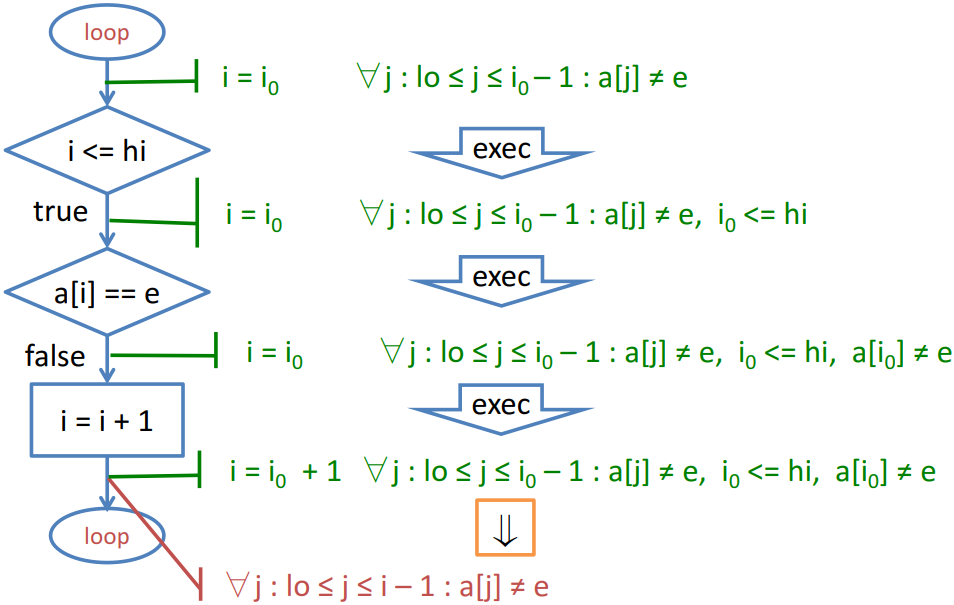
\includegraphics[width=0.5\textwidth,keepaspectratio]{symbolic_execution}
\end{figure}

\section{Discuss contract-based reasoning on procedures and data structures}

\begin{itemize}
    \item \textblue{On procedure} : Compositional reasoning\\
    Follow the hierarchical structure of a program :
    \begin{itemize}
        \item At a small scale (within a single procedure)
        \item At a larger scales (across multiple procedure ...)
    \end{itemize}
    \textblue{Hoare triple} : [pre] block [post]
    \begin{itemize}
        \item  if pre is satisfied at the entry to the block, then the post should be satisfied after execution of the block
        \item[$\Rightarrow$] Summarize the effect of a block of program by a contract [pre] block [post]
        \item[$\Rightarrow$] Prove that block satisfies pre/post then use the contract wherever the block is used
    \end{itemize}

    \item \textblue{On data structures} :\\
    Data structure module $=$ data (encapsulated) + operations = variables + procedures (methods)\\
    Contract $=$ 
    \begin{enumerate}
        \item \textblue{Abstraction function} "abs" : relates data structures D to an abstract model abs(D) (e.g. abs : Dictionary $\rightarrow$ {<key, value>})
        \item \textblue{Structural invariant} "ok" : data structure characteristics that must be maintained (e.g. ok : Dictionary $\rightarrow$ bool)
    \end{enumerate}
    Contract for Dictionary.get :
    \begin{itemize}
        \item[] \textit{{[<k,v> in abs(dict) and ok(dict)]}}
        \item[] \textit{o = dict.get(k)}
        \item[] \textit{{[o = v and ok(dict)]}}
    \end{itemize}
\end{itemize}

\chapter{Program analysis}

\section{Describe the principles of program inspection, static and dynamic program analysis}

\begin{enumerate}
    \item \textblue{Program inspection} : Systematic, detailed review of artifacts (= code but also specifications, documentation, tests, ...) to find defects and assess quality.\\ 
    Used for :
    \begin{enumerate}
        \item Find and remove defects
        \item Incentive to produce good code
        \item Share coding norms and practices
        \item Familiarize new staff with the code
    \end{enumerate}
    \textblue{Team}: the programmer(s) + experts (+ usage of \textblue{checklist})\\
    With different perspectives : junior and senior engineers, testers, managers, analysts, architects, ...\\
    Moderator: external senior manager
    \item \textblue{Static analysis} : examine source code. Examine the complete execution space but may lead to false alarm
    \item \textblue{Dynamic analysis} : examine execution traces. No infeasible path problem but cannot examine the execution space exhaustively
\end{enumerate}

\section{Explain symbolic testing and its application to pointer analysis}

\textblue{Symbolic testing} : 
\begin{itemize}
    \item Abstract variables with \textblue{few symbolic values}
    \item Apply \textblue{symbolic execution}
    \item \textblue{No need} to follow \textblue{all paths}
    \begin{itemize}
        \item Explore paths to a limited depth
        \item Prune exploration by some criterion
    \end{itemize}
    \item Sensitivity :
     \begin{itemize}
        \item Symbolic testing is \textblue{path sensitive}: different symbolic states from paths to the same location
        \item Symbolic testing is \textblue{partly context sensitive}: different symbolic states implies different call sequences
        \item This is a strength of symbolic checking
        \begin{enumerate}
            \item Detailed description of how fault is reached
            \item Costly
            \item Reduce costs by memorizing entry and exit conditions
        \end{enumerate}
    \end{itemize}
    \item Example (\textblue{pointer analysis}) : every \textblue{pointer variable} is represented by a \textblue{machine} with three states.\\
    Possible errors : deallocation in \textit{maybe null}, dereference in \textit{maybe null} and dereference in \textit{invalid}.
\end{itemize}

\begin{figure}[H]
    \centering
    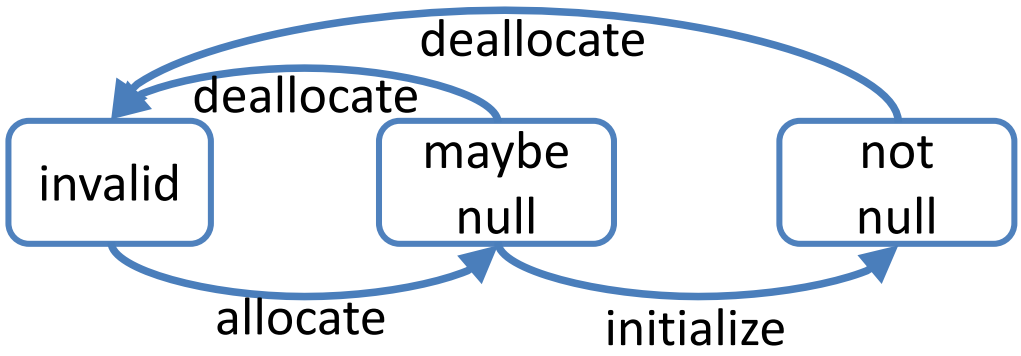
\includegraphics[width=0.5\textwidth,keepaspectratio]{pointer_analysis}
\end{figure}

\section{Explain dynamic analysis and its application to lockset analysis}

\textblue{Dynamic program analysis} :
\begin{itemize}
    \item Track program execution
    \begin{itemize}
        \item Instrument program to trace memory accesses
        \item Record the state of each memory location
        \item Detect accesses incompatible with the current state
        \begin{itemize}
            \item Access unallocated memory
            \item Read from uninitialized memory
            \item Array bounds violations
        \end{itemize}
    \end{itemize}
    \item Amplify sensitivity of testing to detect potential data races (two threads access a location, and at least one is a write, and there is no lock protecting that location).
\end{itemize}

\textblue{Lockset analysis} :
\begin{itemize}
    \item \textblue{Lockset discipline} : Every shared variable must be protected by a lock
    \item \textblue{Dynamic lockset analysis} : detects violation of the locking discipline
    \item \textblue{Algorithm} :
    \begin{lstlisting}[style=pseudoCode, escapeinside=@@]
Identify set of locks held by threads when accessing each shared variable.
For each variable x, a set Lockset(x)
INIT: Lockset(x) = {all locks}
thread A accesses x: Lockset(x) = Lockset(x) @$\bigcap$@ Locks(A)
END: if Lockset(x) = {} report ERROR (no lock consistently protects v)
    \end{lstlisting}
\end{itemize}

\begin{figure}[H]
    \centering
    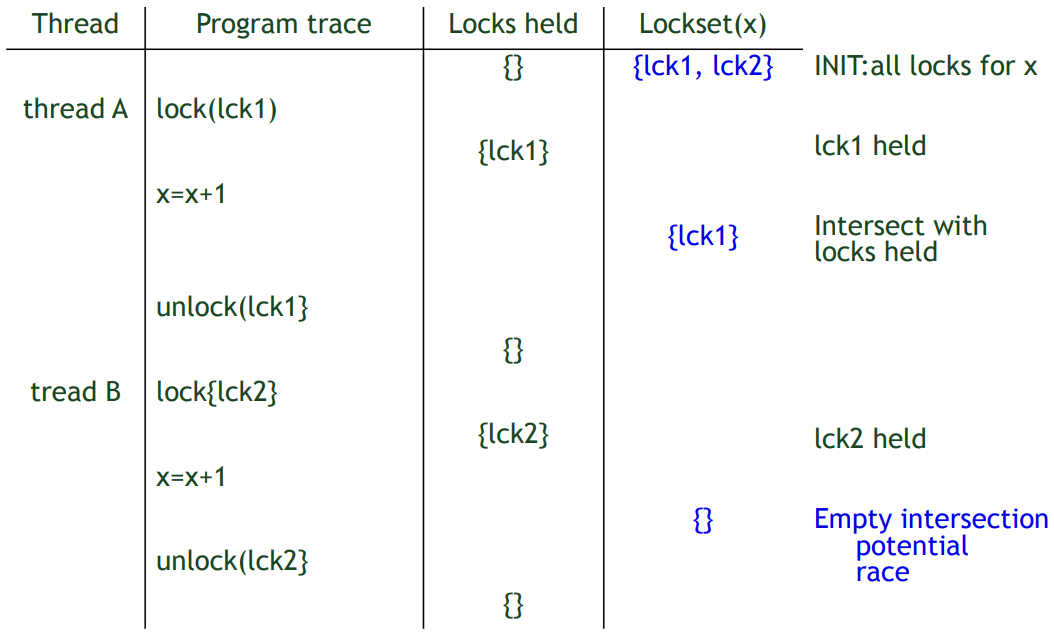
\includegraphics[width=0.7\textwidth,keepaspectratio]{lockset_analysis}
\end{figure}

\chapter{Finite state analysis I}

\section{Describe the principles of finite-state analysis}

\textblue{Finite state verification} :
\begin{itemize}
    \item Prove some significant properties on a finite model of the infinite execution space
    \item Techniques from symbolic execution and formal verification
    \item Iterative process :
    \begin{enumerate}
        \item Prepare a model and specification
        \item Repeat :
        \begin{enumerate}
            \item Attempt verification
            \item Receive reports of impossible or unimportant faults
            \item Refine the specification and/or the model
        \end{enumerate}
        \item Until no impossible or unimportant faults
    \end{enumerate}
    \item Is complementary to testing (can find bugs that are extremely hard to test for {[concurrency, race conditions]} but is limited in scope)
\end{itemize}

\section{Define safety and liveness properties and discuss their verification}

\begin{minipage}[t]{0.48\textwidth}
    \textblue{Safety} :
    \begin{itemize}
        \item Bad things should not happen\\
        Example :
        \begin{enumerate}
            \item Invariant violation, assertion violation
            \item Mutual exclusion: two process should not modify a variable at the same time
            \item [3.] [P] S [Q]: partial correctness
        \end{enumerate}
        \item Specify with \textit{assert(...)}
        \item \textblue{Verify with reachability (easy)}    
    \end{itemize}
    \begin{figure}[H]
        \centering
        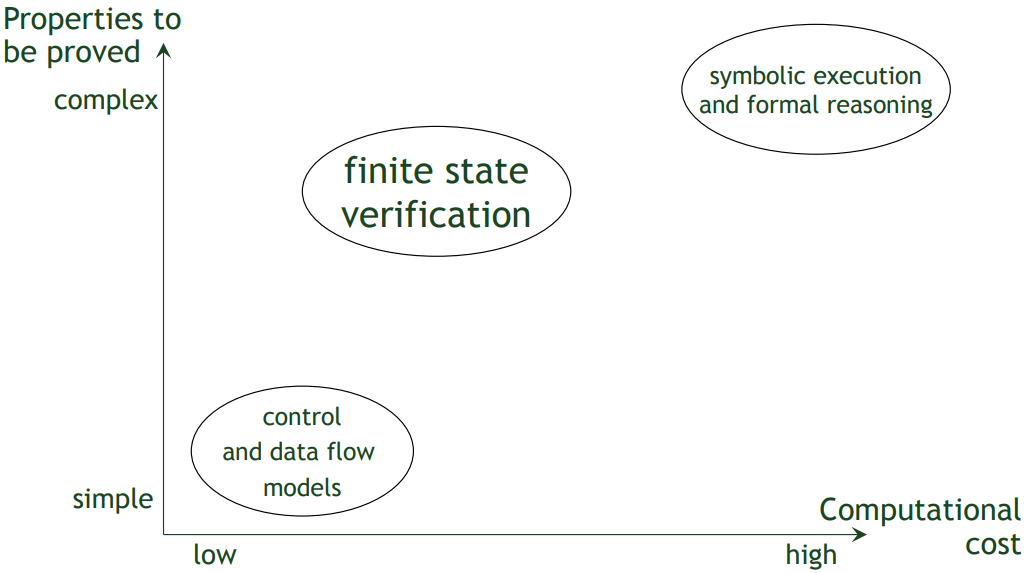
\includegraphics[width=\textwidth,keepaspectratio]{safety_reachability}
    \end{figure}
\end{minipage}
\hfill
\begin{minipage}[t]{0.48\textwidth}
    \textblue{Liveness} :
    \begin{itemize}
        \item Good things should eventually happen\\
        Examples : 
        \begin{enumerate}
            \item Response : if I push the button, eventually the elevator should arrive
            \item Fairness : all enabled threads get executed
            \item Program termination
        \end{enumerate}
        \item Specify in \textblue{temporal logic}
        \begin{figure}[H]
            \centering
            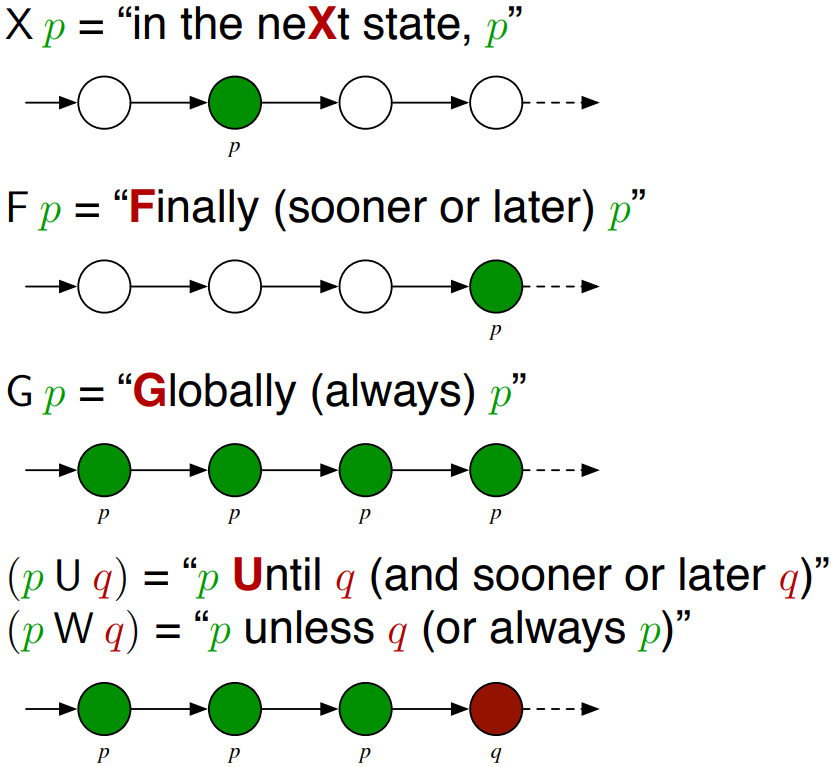
\includegraphics[width=0.6\textwidth,keepaspectratio]{temporal_logic}
        \end{figure}
        \item Verify with automata, repeated reachability (more expensive)
    \end{itemize}
\end{minipage}

\newpage
\section{Discuss the model size and correspondence problems}

\begin{enumerate}
    \item \textblue{State explosion} : the \textblue{size of the state model} grows very quickly and can become too large.\\
    With $\#K$ processes and $\#N$ states each, the number of global states is : $\#K^{\#N}$
    \item \textblue{Model correspondence problem} : consistency between model and program?
    \begin{enumerate}
        \item \textblue{Model extracted from the program}
        \begin{itemize}
            \item [$\Rightarrow$] Verify the \textblue{extraction} procedures (once for all)
            \item Challenge: right level of detail
            \begin{enumerate}
                \item All details $\Rightarrow$ state space explosion
                \item Missing details $\Rightarrow$ "false alarm" reports
            \end{enumerate}
        \end{itemize}
        \item \textblue{Program generated from the model}
        \begin{itemize}
            \item [$\Rightarrow$] Verify the \textblue{generation} procedures (once for all)
        \end{itemize}
        Most applicable within well-understood domains
        \item \textblue{Model written (partially or entirely) by hand}
        \begin{itemize}
            \item [$\Rightarrow$] Check \textblue{conformance} by (model-based) testing
        \end{itemize}
    \end{enumerate}
\end{enumerate}

\chapter{Finite state analysis II}

\section{Explain intensional representations for finite state analysis and describe the use of binary decision diagrams}

Enumerating (and storing) all reachable states costs a lot, it is a limiting factor of finite state verification. The alternative is to use intensional (symbolic) representations which describes sets of reachable states without enumerating each one individually.
\begin{itemize}
    \item Intensional representations may be more compact than the set they represent
    $$\{x \in N | x\  mod \ 2 = 0 \wedge 0 < x < 1000  \} \rightarrow 500\  elem$$
    This is only because of structure or regularity in the set that is captured by the representation !
    \item Unstructured, irregular sets will necessarily have a larger intensional representation
    \item \textblue{Information theory} : representing subsets of N elements ($2^N$ possibilities) requires \bigO$(N)$ in average
\end{itemize}

\textblue{Binary decision diagrams (BDDs)} are a type of intensional model and a compact representation of Boolean functions. A BDD $=$ a binary decision tree with a fixed order on the variables with merged identical subtrees. Operations can be efficiently computed on BDDs.

\section{Discuss iterative model refinement}

Construction of finite state models (balancing precision and efficiency).\\
Often the first model is unsatisfactory
\begin{itemize}
    \item Report unfeasible failures
    \item Exhaust resources before producing any result
    \item [$\Rightarrow$] Idea : improve the model and restart (finite state verification as iterative process)
\end{itemize}

\begin{figure}[H]
    \centering
    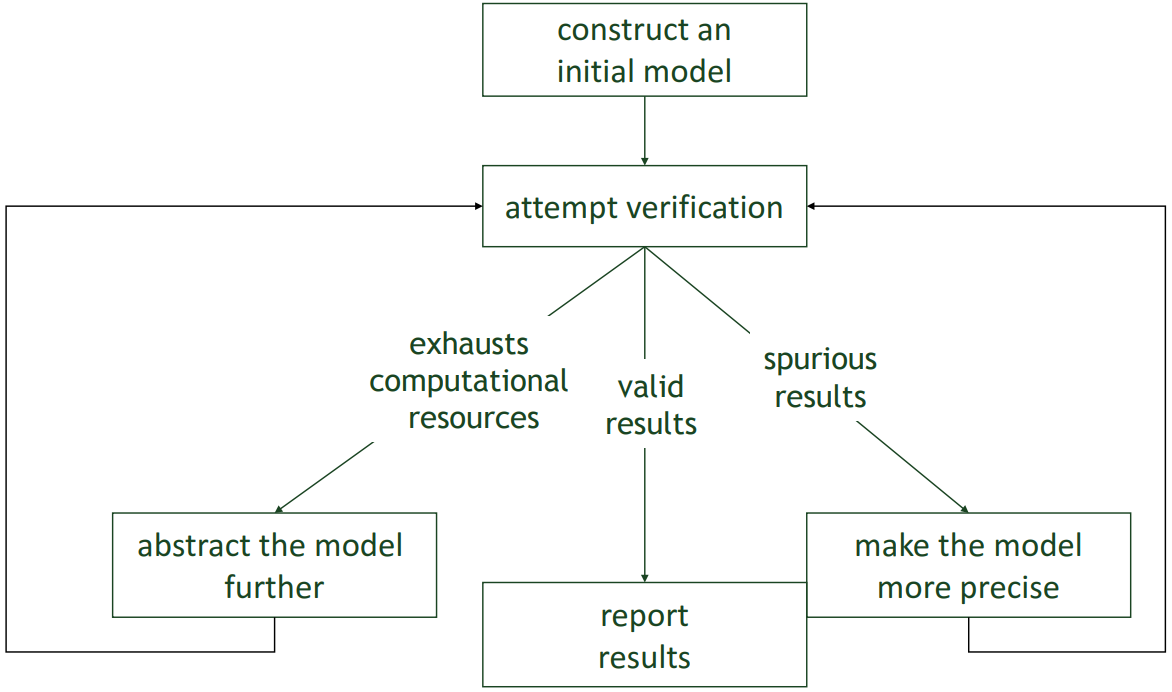
\includegraphics[width=0.5\textwidth,keepaspectratio]{iterative_process}
\end{figure}

\newpage
\section{Describe the principles of data model verification}

Many information systems are characterized by 
\begin{enumerate}
    \item simple program logic and algorithms
    \item complex data structures
\end{enumerate}
A key element is the data model (class and object diagrams + OCL assertions) = sets of data and relations among them.

Challenge : prove that 
\begin{enumerate}
    \item Individual constraints are consistent
    \item Together they ensure the desired properties of the system as a whole
\end{enumerate}

In a complex data models, we use the same general verification principles
\begin{enumerate}
    \item systematic analysis of models
    \item thorough testing is impractical
\end{enumerate}
The difficulty is to consider all the possible combinations of choices in a complex data model. (take the website as an example)

\chapter{Software measurement: size}

\section{State the general principles of software measurement}

\textblue{Principles} :
\begin{itemize}
    \item \textblue{Software measurement} : deriving a numeric value of a property of a software product or a process. (To allow comparison)
    \item \textblue{Measurement} (more general) : mapping from the empirical world to the formal world.
    \item \textblue{Metrics} : a means of measurement of a property of a software product or a process.
    \item \textblue{Objective} : understand, control and improve the quality of a software.
    \item \textblue{Attributes} :
    \begin{enumerate}
        \item \textblue{Internal} (structural) : size, complexity
        \item \textblue{External} (functional) : quality, reliability
    \end{enumerate}
\end{itemize}

\section{Discuss size measurement metrics based on lines of code}

\textit{Note} : A size measurement should be non-negative, zero iff empty and additive.

There are different size metrics: lines of code, number of bytes, number of modules.... The choice of measure is made according to the question to be answered (complexity, disk footprint,...)

\textblue{Line Of Code ($LOC$)} $\rightarrow$ How to count them ? What about blank lines, comments, data declarations, several instructions on a line
\begin{itemize}
    \item \textblue{$NCLOC$} : No Commented $LOC$. (No commented line, no blank line, everything else counts as 1 per line)
    \item \textblue{$CLOC$}: Commented $LOC$. (Line commented)
    \item [$\Rightarrow$] \textblue{$LOC$} $= NCLOC + CLOC$
    \item [$\Rightarrow$] \textblue{Comment Density} $= CLOC / LOC$
\end{itemize}
\noindent What count ? What files ? 
\begin{enumerate}
    \item Which files ? 
    \begin{itemize}
        \item [$\Rightarrow$]Program code, test drivers, automatically generated code, imported code
    \end{itemize}
    \item Which code ? the delivered or the developed ?
    \begin{itemize}
        \item \textblue{Executable Statement ($ES$)} : No blank, no comments, no data nor headers, 1 per statement.
        \item \textblue{Delivered Source Instruction ($DSI$)} : No blank, no comment, 1 per statement or data declaration
    \end{itemize}
\end{enumerate}

\section{Explain functional size measurement using function points}

\textblue{Function point ($FP$)} : measures the amount of functionality.\\
Useful to : 
\begin{enumerate}
    \item Estimate the development effort and duration ($mm/FP$)
    \item Express defect density ($\#defects/FP$)
    \item Bill the development ($\$/FP$)
\end{enumerate}

\newpage
\textblue{Example : Spell-checker spec}\\
The checker accepts as input a document file and an optional personal dictionary file. The checker lists all words not contained in either of these files. The user can query the number of words processed and the number of spelling errors found at any stage during processing.

\begin{itemize}
    \item \textblue{Point 1} : Number of items
    \begin{itemize}
        \item $A$ : external files (file names, menu selection)
        \item $B$ : external output (report message)
        \item $C$ : external inquiries (interactive inputs requiring a response)
        \item $D$ : external files (interfaces to other systems)
        \item $E$ : internal files (master files in the system)
    \end{itemize}
    \begin{figure}[H]
        \centering
        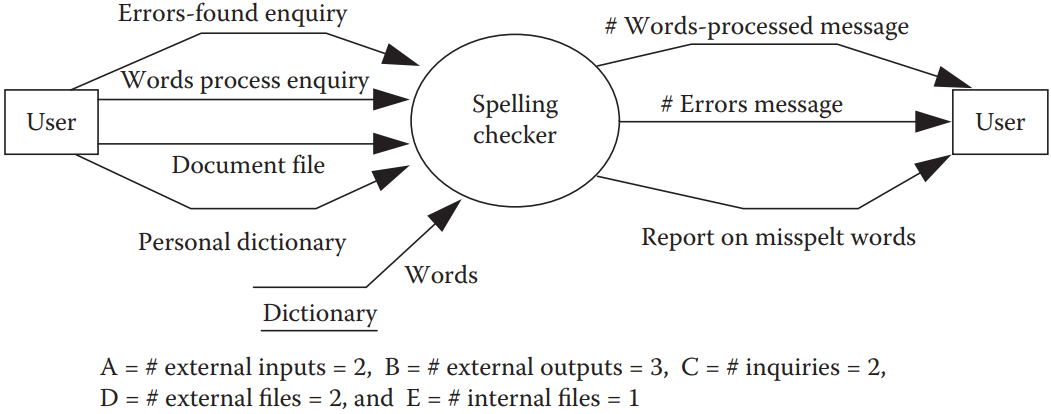
\includegraphics[width=0.5\textwidth,keepaspectratio]{function_point_1}
    \end{figure}
    
    \item \textblue{Point 2} : Complexity for each item (weight)\\
    Unadjusted function points :
    $$UFC = \sum(\#item\ of\ type\ i) * (weight\ of\ type\ i)$$
    \begin{figure}[H]
        \centering
        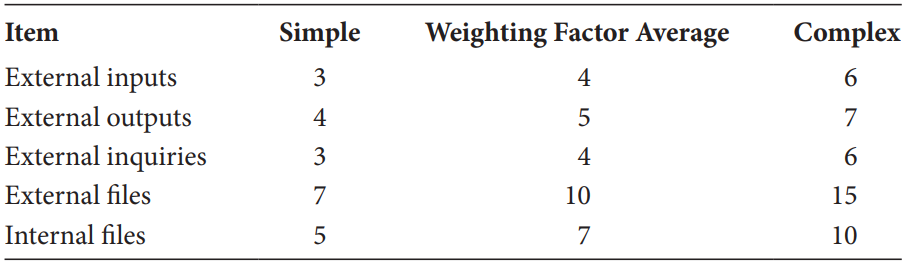
\includegraphics[width=0.5\textwidth,keepaspectratio]{function_point_2}
    \end{figure}
    Example : all average complexity
    \begin{itemize}
        \item $A = 2,\ B = 3,\ C = 2,\ D = 2,\ E = 1$
        \item $UFC = 4 A + 5 B + 4 C + 10 D + 7 E = 58$
    \end{itemize}
    \item \textblue{Point 3} : Technical complexity factors (TFC)\\
    Each $F_i$ is between $0$ and $5$ :
    \begin{itemize}
        \item $TFC = 0.65 + 0.01 \sum F_t$
        \item $FP = UFC * TFC$
    \end{itemize}
    \begin{figure}[H]
        \centering
        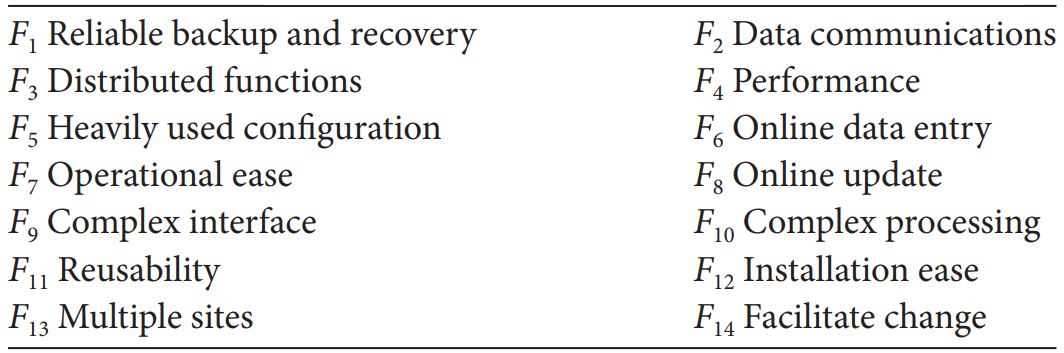
\includegraphics[width=0.5\textwidth,keepaspectratio]{function_point_3}
    \end{figure}
    Example : $6$ factors at $0$, $6$ factors at $3$, $2$ factors at $5$
    \begin{itemize}
        \item $TCF = 0.65 + 0.01 (6 * 3 + 2 * 5) = 0.93$
        \item $FP = 58 * 0.93 = 54$
    \end{itemize}
\end{itemize}

\chapter{Software measurement: structure}

\section{Describe the principles of structure measurement}

The \textblue{size} doesn't tell everything, the \textblue{structure} plays a very important role too to capture the \textblue{complexity} of the product. The structure measurement is applicable to design or code seen as a graph.

\textblue{Two perspectives} :  Control Flow \& Data Flow

Structural attributes : 
\begin{enumerate}
    \item \textblue{Complexity} : complicatedness of the connections between elements in a system model (positive, monotonic, additive on disjoints elements)
    \item \textblue{Length} : distance between elements (positive, monotonic, max on disjoints elements)
    \item \textblue{Coupling} : links to/from the elements outside the module (positive, monotonic, at most sum on merged modules)
    \item \textblue{Cohesion} : connections between internal elements (0 to 1, monotonic, at most sum on merged modules)
\end{enumerate}

\section{Describe hierarchical measures based on prime decomposition of control flow graphs}

\begin{itemize}
    \item \textblue{Control flow graph} : a graph with distinguished start and stop nodes. We want measures that are independent of a particular view (granularity) of the graph
    \item \textblue{Prime decomposition} : A structured flow graph can be decomposed into primes (corresponds to a structured program construction). The decomposition is unique, can be done automatically and allows to check whether a program is S-structured (we decompose into primes and we check if all primes are in S).\\
    Given a family S of prime flowgraphs, a flow graph is S-structured iff it is generated from S by a finite number of sequencing and nesting.
    \begin{figure}[H]
        \centering
        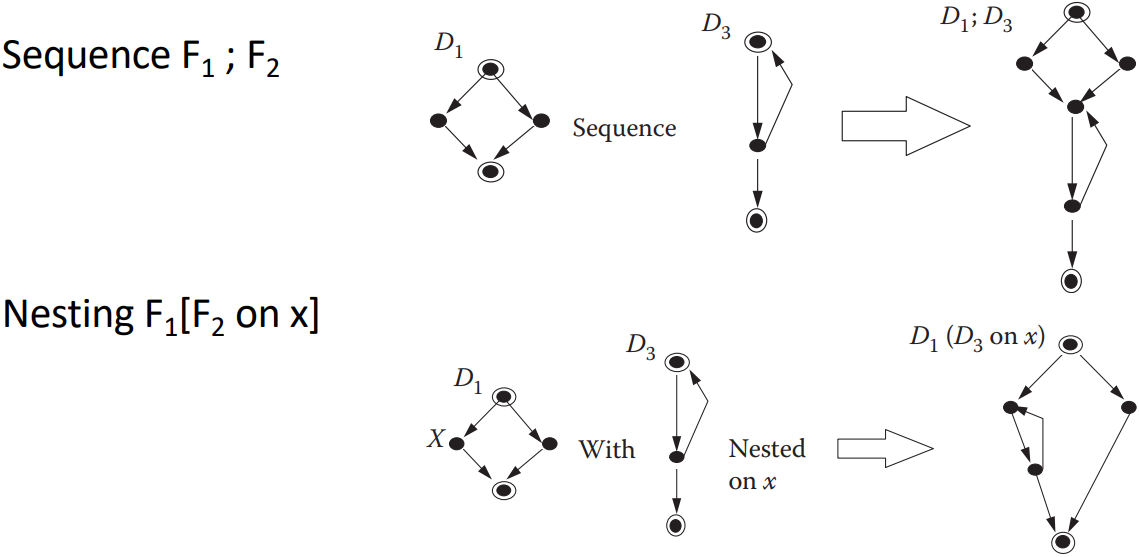
\includegraphics[width=0.6\textwidth,keepaspectratio]{sequencing_nesting}
    \end{figure}
    \item \textblue{Prime flow graph}: a graph that cannot be decomposed by sequencing or nesting
    \item [$\Rightarrow$]\textblue{Hierarchical measures}: measures defined on the prime decomposition tree.\\
    For example: depth of nesting.
    \begin{figure}[H]
        \centering
        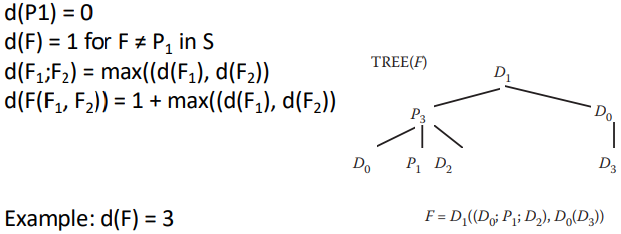
\includegraphics[width=0.5\textwidth,keepaspectratio]{hierarchical_ex1}
    \end{figure}
    More generally, we define :
    \begin{enumerate}
        \item $M_1$ : $M(F)$ for each $F$ in $S$
        \item $M_2$ : $M(F_1;...;F_n)$ from $M(F_i)$
        \item $M_3$ : $M(F(F_1,...,F_n$)) from $M(F_i)$
        \item [$\Rightarrow$] $M_1$, $M_2$, $M_3$ gives hierarchical measures (ex: size $v(F) \equiv$ number of nodes)
    \end{enumerate}
    Example for size $v(F)$ (number of nodes)
    \begin{itemize}
        \item $M_1$ : $v(P_1) = 1$, and for each prime $F \neq P_1$, $v(F) = n+1$, where $n$ is the number of procedure nodes in $F$
        \item $M_2$ : $v(F_1; ...; F_n) = \sum v(F_i)$
        \item $M_3$ : $v(F(F_1, ..., F_m)) = 1 + \sum v(F_i)$ for each prime $F \neq P_1$
    \end{itemize}
\end{itemize}


\section{Define cyclomatic complexity measure}

\begin{itemize}
    \item \textblue{Basis set} : a maximal set of linearly independent paths (any path is a linear combination of paths from the basis set)
    \item \textblue{Cyclomatic number}: the number of path in a basis set.
    $$v(CFG)= \#edges - \#nodes + 2 = \#decision\ points + 1$$
    \begin{figure}[H]
        \centering
        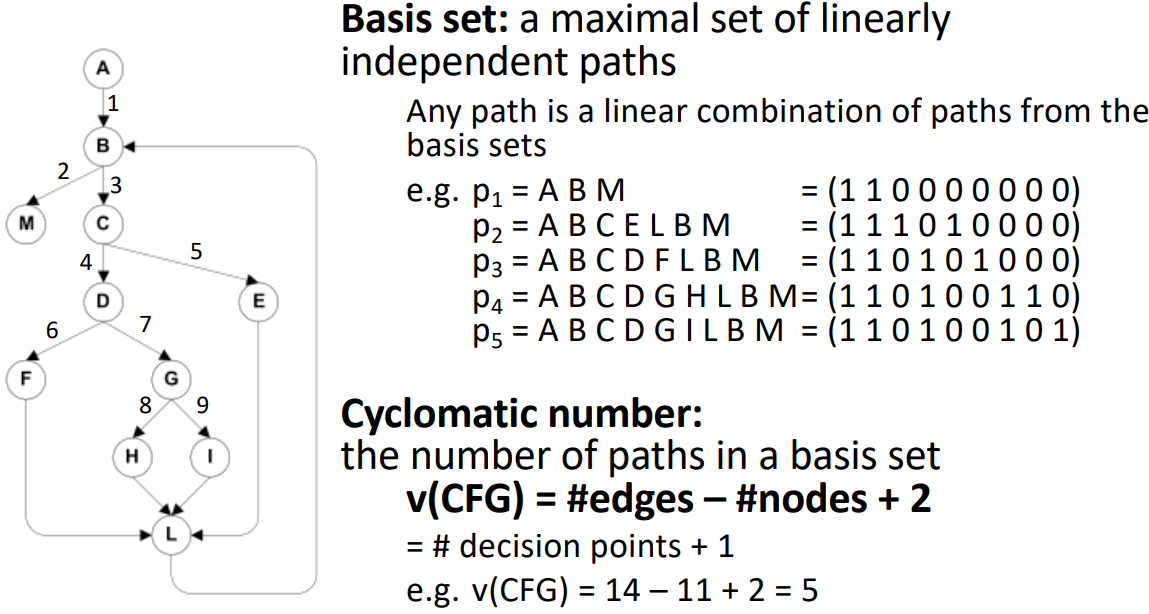
\includegraphics[width=0.5\textwidth,keepaspectratio]{cyclomatic_number}
    \end{figure}
    \item Cyclomatic complexity is hierarchical
    \begin{itemize}
        \item $M_1$ : $v(D) = 1 + d$, for each prime $F$, where $d$ is the number of predicates in $F$
        \item $M_2$ : $v(F_1; ...; F_n) = \sum_{i=1}^n v(F_i) - n + 1$ for each $n$
        \item $M_3$ : $v(F(F_1, ..., F_m)) = v(F) + \sum_{i=1}^n v(F_i) - n$ for each prime $F$
    \end{itemize}
\end{itemize}

\section{Discuss design-level, inter-modular complexity measures}

So far we have talked about intra-modular measures (inside a procedure). Now we will present inter-modular measures (dependencies between modules). We thus consider design (module structure is the same for code).

\textblue{Dependency graphs} : graph representing the dependency between modules (information flow or call graph). Inside modules we have data dependency graphs.
\begin{figure}[H]
    \centering
    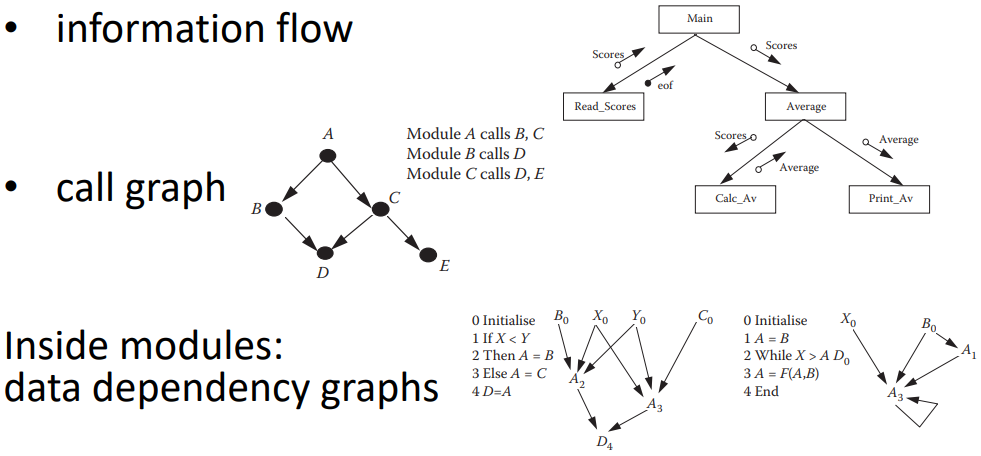
\includegraphics[width=0.55\textwidth,keepaspectratio]{dependency_graph}
\end{figure}

\chapter{Software measurement: quality}

\section{Describe the principles and elements of quality models}

The question here is: Does a product have desirable attributes? (A product can be a document, a file, a system,... while an attribute can be completeness, consistency, reliability,...). Product quality models give a hierarchical nomenclature of product quality characteristics.

A quality models has different elements :
\begin{figure}[H]
    \centering
    \includegraphics[width=0.55\textwidth,keepaspectratio]{quality_model}
\end{figure}


There are different models such like McCall's (left) or Boehm's (right) quality model which are \textblue{fixed models}.
\begin{figure}[H]
    \centering
    \includegraphics[width=0.49\textwidth,keepaspectratio]{mccall_model}\hfill
    \includegraphics[width=0.49\textwidth,keepaspectratio]{boehm_model}
\end{figure}

\newpage
\textblue{But we can also define our own models} :
\begin{itemize}
    \item Keep general philosophy of quality models (factors, criteria, metrics)
    \item Select attributes suited for a particular product
    \begin{itemize}
        \item Discuss with customers, users
        \item Possibly taken from some fixed model
    \end{itemize}
    \item Refine to criteria, metrics
\end{itemize}

\textblue{We can design it by measurable objectives} :
\begin{itemize}
        \item Measurable attributes identified in the specification
        \item Applicable to small, evolutionary development, agile processes
\end{itemize}
\begin{figure}[H]
    \centering
    \includegraphics[width=0.5\textwidth,keepaspectratio]{standard_model}
\end{figure}

\section{Discuss defect-based quality measures}

We take a narrow view : 
\begin{enumerate}
    \item \textblue{Quality} = lack of defects
    \item \textblue{Defects} = errors, faults, failures
\end{enumerate}
There are known defects (from testing, inspection,...) and latent defects (unknown). 
$$defect\ density = \frac{\#know\ defects}{product\ size}$$

From this equation, one need to define what counts as defects (faults, failures, post-test, post-release,...) and what counts as size (comments, data binaries, tests,...). It is also important to not confuse with
defect rate which is relative to time and not size.

There are different type of defect-based measures, another example :
$$Spoilage = \frac{time\ to\ fix\ defects}{total\ dev\ time}$$

\section{Discuss usability, maintainability and security measures}

\textblue{Usability} :

The degree to which a product or system can be used by specified users to achieve specified goals with effectiveness, efficiency and satisfaction in a specified context of use.

\textblue{Example} : User-friendliness (ease to learn, use, remember) or user satisfaction.\\
$\Rightarrow$ This is not a directly measurable attribute, so we need to define usability measurements
\begin{itemize}
    \item \textblue{Effectiveness} : \% of correctly completed tasks. User recall = remember information provided (task effectiveness = quantity x quality of tasks)
    \item \textblue{Efficiency} : time to complete a task, input rate
    \begin{itemize}
        \item time efficiency = effectiveness / task time
        \item productive period = productive time / task time
        \item relative user efficiency = user efficiency / expert efficiency
    \end{itemize}
    \item \textblue{Satisfaction} : questionnaires, biological measurements
\end{itemize}

Other usability measurements, not in ISO 25010 :
\begin{itemize}
    \item \textblue{Accessibility} : disabilities (visual, hearing, physical)
    \item \textblue{Universality} : cultural norms, naming conventions
    \item \textblue{Trustfulness} : trust of users in the system ($\rightarrow$ security)
\end{itemize}

Internal elements related to usability:
\begin{itemize}
    \item Good use of menus and graphics
    \item Informative error messages
    \item Help functions
    \item Consistent interfaces
    \item Well-structured manuals
\end{itemize}

Size and structure can also be measured. In particular, text structure affects readability and comprehensibility. But size and structure are poor measures of quality.

\textblue{Maintainability} :

The degree of effectiveness and efficiency with which a product or system can be modified by the intended maintainers. Easy to understand, enhance and correct. Maintenance can be :
\begin{itemize}
    \item Corrective (fix bugs)
    \item Adaptive (changes, upgrades)
    \item Preventive (before failures occur)
    \item Perfective (enhance, extend)
\end{itemize}

They apply to code, documentation, specs, design, tests,... Maintenance is about making changes to the product. There are different maintainability measures :
\begin{itemize}
    \item (\textblue{Most important one}) \textblue{Mean Time To Repair (MTTR)}: average time to implement a change and restore the system to working order, can be split in different measure times :
    \begin{itemize}
        \item Problem recognition time
        \item Administrative delay time
        \item Maintenance tools collection time
        \item Problem analysis time
        \item Change specification time
        \item Change time (including testing and review) 
    \end{itemize}
    \item Change time/number of changes
    \item Number of unresolved problems
    \item Time spent on unresolved problems
    \item \% changes that introduce new faults
    \item Number of modules modified for a change
\end{itemize}

Concerning internal elements related to maintainability:
\begin{itemize}
    \item \textblue{Structural complexity} : this is more an indication, not really a measure. Used in correlation with external measures (e.g. identify a module with poor structure)
    \item Readability : for texts, we can use the Fog Index
\end{itemize}


\textblue{Security} :

The degree to which a product or system protects information and data so that persons or other products or systems have the degree of data access appropriate to their types and levels of authorization.\\
No "competent programmer" hypothesis: assume that attackers try to overcome security protections and hide their activities.

Security measures :
\begin{enumerate}
    \item \textblue{Risk} = Impact $\times$ Likelihood $\times$ Threat $\times$ Vulnerability (where impact, likelihood and vulnerability depend on threat).
    \item \textblue{Common vulnerability Scoring System (CVSS)} gives a metric between 0 and 1 based on 6 measures. $\textblue{CVSS} = f(AV, AC, Au, C, I, A)$
    \begin{enumerate}
        \item Access vector ($AV$) : how remote an attacker can be
        \item Access complexity ($AC$): how complex the attack needs to be
        \item Authentication ($Au$) : how many authentications needed
        \item Confidentiality impact ($C$) : impact to system information confidentiality
        \item Integrity impact ($I$) : impact to system integrity
        \item Availability impact ($A$) : reduced performance, shutdown
    \end{enumerate}
    \item \textblue{Bayesian analysis (probabilistic)} : based on attack probabilities and costs
    \item \#vulnerabilities / \#defects
\end{enumerate}

\noindent \textblue{Internal measures} : Number of entry points, exit points, data channels, persistent data items

\chapter{Software reliability}

\section{Describe the model of reliability based on failure rates}

Reliability is a key quality attribute: top-level in all quality models and the most extensively studied.
Reliability has as objectives :
\begin{enumerate}
    \item Measure failures
    \item Predict future failures from past failures
    \item Reliability growth: predict reliability from past faults found and fixed
    \item[$\Rightarrow$] Want to answer a basic question : When will the system fail?
\end{enumerate}


Software failures are different from hardware failures. A component may fail due to physical wear. The probability that the component will fail at time $t$ is given by the probability density function $f(t)$

\section{Define failure probability functions, reliability, maintainability, availability, MTTF and MTTR}

\begin{itemize}
    \item Failure probability \textblue{density function} is the probability that a failure will occur between time $t$ and time $t+dt$ :\\
    $f(t)dt=Prob$(failure between $t$ and $t+dt$)
    \item Failure probability \textblue{distribution function} is the probability that a failure will occur between 0 and $t$ :\\
    $F(t)=\int f(t)dt =$ Prob(failure between $0$ and $t$)
    \item \textblue{Reliability} : operating without failure for a given time interval. It is time-dependent :\\
    $R(t) = 1-F(t)$ = Prob(no failure before $t$)
    \item \textblue{Maintainability} : maintenance activity can be carried out within stated time interval, procedures and resources. Also time-dependent :\\
    $M(t)$ = Prob(restored before $t$)
    \item \textblue{Availability} : operation without failure at a given point in time, time-independent.\\
    $A=Prob(not \ failed)= MTTF/(MTTF+MTTR)$
    \item \textblue{MTTF} : Mean Time To Failure is the average time before failure occurs. It measures reliability.
    \item \textblue{MTTR} : Mean Time To Repair is the average time to fix a fault. It measures maintainability.
\end{itemize}

\section{Describe the case of constant failure rates}

\textblue{Constant failure rate}: it is when the software will fail purely randomly independently of the past, no memory. We have a constant probability rate $\lambda$.
\begin{enumerate}
    \item $f(t)= \lambda exp(-\lambda t)$
    \item $F(t) = 1-exp(-\lambda t)$
    \item $R(t)= exp(-\lambda t)$
\end{enumerate} 

\chapter{Failure prediction}

\section{Describe the principles of failure prediction systems}

\begin{itemize}
    \item Given a series of failure times $(t_1, t_2, ..., t_i-1)$ where the fault has been fixed after each failure. The goal of these systems is to predict future failure times $T_i, T_{i+1},....$
    \item In software, as we fix faults, we expect the reliability to grow.
    \item The \textblue{goal of a prediction system} is to predict the probability distributions $F_i, F_{i+1},...$
    \item A \textblue{prediction system} has three elements :
    \begin{itemize}
        \item \textblue{Prediction model} : probability specification of the stochastic process (distributions $F_i(T_i)$)
        \item \textblue{Inference procedure} : infer unknown parameters of the model from $t_1, t_2, ..., t_{n-1}$
        \item \textblue{Prediction procedure} : combine the model and inference procedure to make predictions about future failure behaviour
    \end{itemize}
\end{itemize}

\section{Discuss the example of the Jelinski-Moranda model}

\begin{itemize}
    \item \textblue{Model} : constant rate $\phi$ identical for all faults
    \begin{figure}[H]
        \centering
        \includegraphics[width=0.45\textwidth,keepaspectratio]{jelinski-moranda_1}
    \end{figure}
    \begin{itemize}
        \item Type-1 uncertainty = random, exponential rate
        \item No type-2 uncertainty = corrections are perfect
        \item Fixing any fault contributes equally to improving the reliability
    \end{itemize}
    \item \textblue{Inference procedure} : maximum likelihood estimation (Gives predictions for $N_i$ and $\phi_i$)
    \item \textblue{Prediction procedure} : predict mean time to next failure ($T_i = 1/\lambda_i = 1/(N_i - i + 1)\phi_1$)
\end{itemize}
\begin{minipage}[t]{0.48\textwidth}
    \begin{itemize}
        \item Example :
        \begin{figure}[H]
            \centering
            \includegraphics[height=\textwidth,keepaspectratio]{jelinski-moranda_2}
        \end{figure}
    \end{itemize}
\end{minipage}
\hfill
\begin{minipage}[t]{0.48\textwidth}
    \begin{itemize}
        \item Criticisms :
        \begin{itemize}
            \item \textblue{Unrealistic assumptions} :
            \begin{itemize}
                \item The sequence of $\lambda_i$ is purely deterministic
                \item All faults equally contribute to the hazard rate
            \end{itemize}
            \item The \textblue{reliability predictions} obtained from the model are \textblue{poor} and usually \textblue{too optimistic}
        \end{itemize}
    \end{itemize}
\end{minipage}

\section{Discuss statistical testing}

\textblue{Idea }: reliability predictions based on failures occurring during testing may not correspond to typical system usage (with different users, tasks, experience levels,...).
\begin{enumerate}
    \item \textblue{Operational Profile} : probability distribution on inputs (reflecting usage)
    \item \textblue{Statistical testing} : select tests according to \textblue{operational profile}
    \begin{itemize}
        \item Tests focus on more used parts $\rightarrow$ better observed reliability
        \item Test reflects usage $\rightarrow$ reliability predictions more accurate.
    \end{itemize}
\end{enumerate}


Operational profiles are difficult to define.\\
$\Rightarrow$ A \textblue{small \% of the operational profil}e may account for a \textblue{large \% of failures}.

Examples :
\begin{enumerate}
    \item Airplane : take-off and landing
    \item Printer : 
    \begin{itemize}
        \item Non-saturated : available, no queue $\rightarrow$ print immediately (20\%)
        \item Saturated : busy, queue $\rightarrow$ add to queue (79\%)
        \item Transitional : busy, no queue $\rightarrow$ create queue and add to queue (1\%)
        \item Probability of failures : 0.001 per test case
    \end{itemize}
    To have a 50\% chance of detecting each fault, me must run :
    \begin{itemize}
        \item Non saturated : 2500 test cases
        \item Saturated : 633 test cases
        \item Transitional : 50 000 test cases
    \end{itemize}
    \item Transitional likely the most complex and failure-prone
\end{enumerate}
